\documentclass[10pt]{article}
\usepackage{NotesTeX} %/Path/to/package should be replaced with package location
\usepackage{lipsum}
\usepackage{tensor}
\usepackage{graphicx,wrapfig,float,slashed,subcaption,bbold,bm}
\usepackage{amsmath,mathtools,amssymb,epsfig,graphicx,xcolor}
\usepackage{epstopdf}
\epstopdfsetup{update}
\usepackage{ragged2e}
\usepackage{mciteplus}
\usepackage[many]{tcolorbox}
\usepackage{pgfplots}
\pgfplotsset{compat=1.5.1}
\usepackage{tikz}
\usetikzlibrary{babel}
\tikzset{>=latex}
\usepackage{hyperref}

\newcommand{\bs}{\textbackslash}
\newcommand{\nc}{\newcommand}
\newcommand{\non}{\nonumber}	
\newcommand{\noi}{\noindent}
\newcommand{\barx}{\bar{x}}
%

\newcommand{\hsp}{\hspace{0.5cm}}
\newcommand{\lsp}{\hspace{1cm}}
\newcommand{\Lsp}{\hspace{2cm}}
%\nnewcommand{\LLsp}{\lsp\lsp}
\newcommand{\lra}{\longrightarrow}
\newcommand{\p}{\prime}
\newcommand{\sgn}{\text{sgn}}
\newcommand{\ph}{\varphi}


\newcommand{\beq}{\begin{equation}}  \newcommand{\eeq}{\end{equation}}
\newcommand{\bea}{\begin{eqnarray}}  \newcommand{\eea}{\end{eqnarray}}
\newcommand{\baa}{\begin{array}}     \newcommand{\eaa}{\end{array}}
\newcommand{\bit}{\begin{itemize}}   \newcommand{\eit}{\end{itemize}}
\newcommand{\ben}{\begin{enumerate}} \newcommand{\een}{\end{enumerate}}
\newcommand{\bce}{\begin{center}}    \newcommand{\ece}{\end{center}}
\newcommand{\bpm}{\begin{pmatrix}}   \newcommand{\epm}{\end{pmatrix}}
\newcommand{\bvt}{\begin{verbatim}}  
\newcommand{\evt}{\end{verbatim}}


\title{{\Huge General Relativity}\\{\Large{Class 9}}} %replace with class number
\author{Asad Hussain}

\emailAdd{asadh@utexas.edu} %replace with your email


\begin{document}
\maketitle
\flushbottom
\newpage
\pagestyle{fancynotes}
    

\part{The Equivalence Principle}

%\section{Recap}
Last time we considered field theory, and how to construct and extract dynamics of the theory of fields: inherently local objects. Our objective is flesh out more of the mathematical machinery necessary to be able to say exact things about generic "local" objects. Before we dive into the math we will introduce some postulates that allow us to connect most of the physics as we have learnt so far to the local ideas we are developing.

\section{The Weak Equivalence Principle}
We know from considering $F = ma$ and $F_g = -mg$, that all objects fall at the same rate, regardless of their mass. There's actually no \textit{apriori} reason as to why these masses should be the same. The $m$ in $F = ma$ (lets call it $m_I$), is the inertial mass, and contains information about the reaction of an object to a force. The $m$ in $F_g = -mg$ (let's call it $m_g$) is sort of the "gravitational charge", and explains how gravitational forces act on it. The fact that $m_I = m_g$ \sn{or at least $m_I \propto m_g$, with the proportionality constant being absorbed into the gravitational constant $G$.}, seems to be an added assumption in the physics of simple Newtonian gravity, and we are going to take it as such. It is a \textbf{postulate}. This leads us to what is known as the weak equivalence principle. \\ 


\begin{tcolorbox}
\textbf{The Weak Equivalence Principle} states that the "inertial mass" $m_I$ is equal to the "gravitational mass" $m_g$
\end{tcolorbox}



We can coax out a new way to formulate this postulate: Let's consider the case when we have two observers, as shown in \textbf{Figure 1}. One in an accelerating reference frame going along in a rocket, and another staying stationary in a gravitational field \sn{Notice how one needs the floor to provide a reaction force of $-\vec{g}$ to an object to prevent it from going into free fall.}.



\begin{figure}[h!]
\centering


\tikzset{every picture/.style={line width=0.75pt}} %set default line width to 0.75pt        

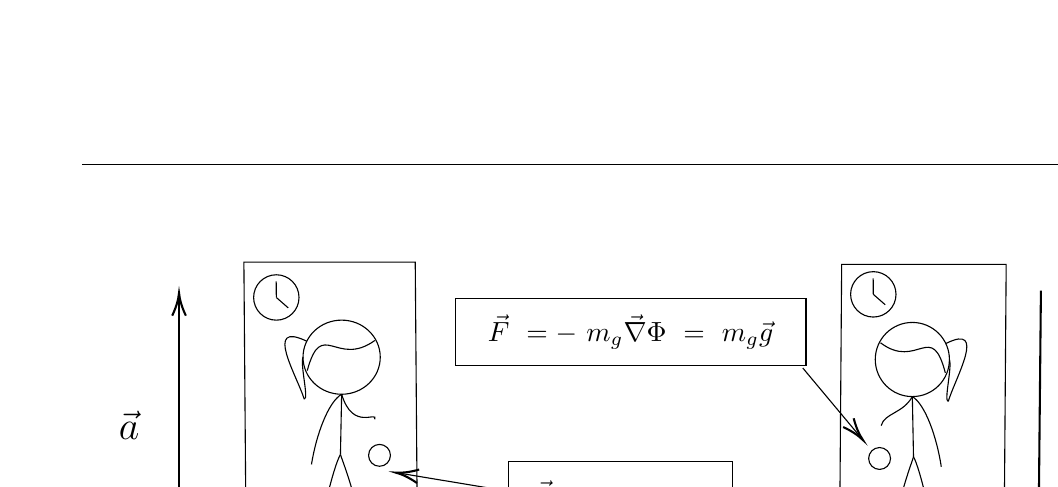
\begin{tikzpicture}[x=0.75pt,y=0.75pt,yscale=-1,xscale=1]
%uncomment if require: \path (0,294.5); %set diagram left start at 0, and has height of 294.5

%Shape: Ellipse [id:dp5247720835968115] 
\draw   (493.42,93.6) .. controls (493.42,83.74) and (501.41,75.74) .. (511.28,75.74) .. controls (521.14,75.74) and (529.14,83.74) .. (529.14,93.6) .. controls (529.14,103.47) and (521.14,111.47) .. (511.28,111.47) .. controls (501.41,111.47) and (493.42,103.47) .. (493.42,93.6) -- cycle ;
%Straight Lines [id:da8134627672975623] 
\draw    (511.28,111.47) -- (511.84,140.49) ;
%Curve Lines [id:da9688542701452454] 
\draw    (511.84,140.49) .. controls (510.72,144.16) and (501.79,167.6) .. (504.02,177.65) ;
%Curve Lines [id:da42282000371090667] 
\draw    (511.84,140.49) .. controls (515.18,146.39) and (520.77,172.81) .. (521.88,178.39) ;
%Curve Lines [id:da2530269422517113] 
\draw    (511.28,111.47) .. controls (517.42,115.13) and (523,130.76) .. (525.23,145.27) ;
%Curve Lines [id:da4520782675840702] 
\draw    (511.28,111.47) .. controls (506.81,119.6) and (497.76,119.45) .. (496.26,125.48) ;
%Curve Lines [id:da3993004957550148] 
\draw    (495.93,85.55) .. controls (513.79,98.95) and (520.49,74.39) .. (527.18,100.06) ;
%Curve Lines [id:da8795957512607879] 
\draw    (527.46,85.89) .. controls (547.56,75.84) and (531.93,102.63) .. (528.58,113.79) ;
%Curve Lines [id:da6952491062370043] 
\draw    (528.58,113.79) .. controls (526.35,113.79) and (530.53,97.29) .. (529.14,93.6) ;
%Shape: Polygon [id:ds5979025111427938] 
\draw   (477.23,47.78) -- (556.49,47.78) -- (555.37,197.37) -- (476.11,197.37) -- cycle ;
%Straight Lines [id:da11423530701251927] 
\draw    (476.11,177.27) -- (555.37,177.27) ;
%Shape: Ellipse [id:dp0294730174322273] 
\draw   (254.92,92.49) .. controls (254.92,82.62) and (246.59,74.63) .. (236.32,74.63) .. controls (226.04,74.63) and (217.71,82.62) .. (217.71,92.49) .. controls (217.71,102.35) and (226.04,110.35) .. (236.32,110.35) .. controls (246.59,110.35) and (254.92,102.35) .. (254.92,92.49) -- cycle ;
%Straight Lines [id:da6747085163283644] 
\draw    (236.32,110.35) -- (235.74,139.37) ;
%Curve Lines [id:da8539342217427686] 
\draw    (235.74,139.37) .. controls (236.9,143.04) and (246.2,166.48) .. (243.88,176.53) ;
%Curve Lines [id:da2528244511267783] 
\draw    (235.74,139.37) .. controls (232.25,145.27) and (226.43,171.69) .. (225.27,177.27) ;
%Curve Lines [id:da9812969421409383] 
\draw    (236.32,110.35) .. controls (229.92,114.02) and (224.11,129.64) .. (221.78,144.16) ;
%Curve Lines [id:da5209902817452925] 
\draw    (236.32,110.35) .. controls (241.76,128.49) and (253.81,117.95) .. (252.3,122.46) ;
%Curve Lines [id:da2279833872834809] 
\draw    (252.31,84.43) .. controls (233.7,97.83) and (226.72,73.27) .. (219.75,98.95) ;
%Curve Lines [id:da6572420705412818] 
\draw    (219.46,84.77) .. controls (198.53,74.72) and (214.81,101.51) .. (218.29,112.68) ;
%Curve Lines [id:da437968359334052] 
\draw    (218.29,112.68) .. controls (220.62,112.68) and (216.26,96.17) .. (217.71,92.49) ;
%Shape: Polygon [id:ds549797097629106] 
\draw   (271.78,46.67) -- (189.22,46.67) -- (190.39,196.25) -- (272.95,196.25) -- cycle ;
%Straight Lines [id:da16999838833780734] 
\draw    (272.95,176.16) -- (190.39,176.16) ;
%Curve Lines [id:da20966345937325803] 
\draw    (225.27,197) .. controls (215.97,205.55) and (218.29,222.3) .. (222.95,232.72) ;
%Curve Lines [id:da11990189580030775] 
\draw    (239.23,195.88) .. controls (253.18,203.69) and (247.36,220.07) .. (241.55,233.83) ;
%Straight Lines [id:da5621928744779998] 
\draw    (241.55,233.83) -- (239.23,212.25) ;
%Straight Lines [id:da4944915696042649] 
\draw    (232.48,253.78) -- (239.23,212.25) ;
%Straight Lines [id:da024279232737980605] 
\draw    (222.95,232.72) -- (227.6,214.48) ;
%Straight Lines [id:da22225061071458807] 
\draw    (232.48,253.78) -- (227.6,214.48) ;
%Straight Lines [id:da9090811913248171] 
\draw [line width=0.75]    (157.97,179.88) -- (157.97,63.55) ;
\draw [shift={(157.97,61.55)}, rotate = 450] [color={rgb, 255:red, 0; green, 0; blue, 0 }  ][line width=0.75]    (10.93,-3.29) .. controls (6.95,-1.4) and (3.31,-0.3) .. (0,0) .. controls (3.31,0.3) and (6.95,1.4) .. (10.93,3.29)   ;
%Straight Lines [id:da9300518916382909] 
\draw [line width=0.75]    (573.23,60.43) -- (572.13,172.3) ;
\draw [shift={(572.12,174.3)}, rotate = 270.56] [color={rgb, 255:red, 0; green, 0; blue, 0 }  ][line width=0.75]    (10.93,-3.29) .. controls (6.95,-1.4) and (3.31,-0.3) .. (0,0) .. controls (3.31,0.3) and (6.95,1.4) .. (10.93,3.29)   ;
%Shape: Ellipse [id:dp5959209877026954] 
\draw   (193.91,63.72) .. controls (193.91,57.68) and (198.81,52.78) .. (204.85,52.78) .. controls (210.89,52.78) and (215.78,57.68) .. (215.78,63.72) .. controls (215.78,69.76) and (210.89,74.65) .. (204.85,74.65) .. controls (198.81,74.65) and (193.91,69.76) .. (193.91,63.72) -- cycle ;
%Straight Lines [id:da5809148230731316] 
\draw    (204.78,55.98) -- (204.85,63.72) ;
%Straight Lines [id:da6549542715820449] 
\draw    (205.62,66.34) ;
%Straight Lines [id:da569085192261527] 
\draw    (204.85,63.72) -- (210.57,68.72) ;
%Shape: Ellipse [id:dp7250739273177036] 
\draw   (481.54,62.21) .. controls (481.54,56.17) and (486.43,51.28) .. (492.47,51.28) .. controls (498.51,51.28) and (503.41,56.17) .. (503.41,62.21) .. controls (503.41,68.25) and (498.51,73.15) .. (492.47,73.15) .. controls (486.43,73.15) and (481.54,68.25) .. (481.54,62.21) -- cycle ;
%Straight Lines [id:da1286223417542367] 
\draw    (492.41,54.47) -- (492.47,62.21) ;
%Straight Lines [id:da20905443139746716] 
\draw    (493.24,64.83) ;
%Straight Lines [id:da5271821709403641] 
\draw    (492.47,62.21) -- (498.2,67.21) ;
%Shape: Circle [id:dp2586501282385272] 
\draw   (249.29,139.78) .. controls (249.29,136.87) and (251.65,134.51) .. (254.56,134.51) .. controls (257.47,134.51) and (259.83,136.87) .. (259.83,139.78) .. controls (259.83,142.69) and (257.47,145.05) .. (254.56,145.05) .. controls (251.65,145.05) and (249.29,142.69) .. (249.29,139.78) -- cycle ;
%Shape: Circle [id:dp7733764873139957] 
\draw   (490.23,141.29) .. controls (490.23,138.38) and (492.59,136.02) .. (495.5,136.02) .. controls (498.41,136.02) and (500.77,138.38) .. (500.77,141.29) .. controls (500.77,144.2) and (498.41,146.56) .. (495.5,146.56) .. controls (492.59,146.56) and (490.23,144.2) .. (490.23,141.29) -- cycle ;
%Straight Lines [id:da20970935140450364] 
\draw    (314.5,156.71) -- (264.32,148.4) ;
\draw [shift={(262.35,148.08)}, rotate = 369.40999999999997] [color={rgb, 255:red, 0; green, 0; blue, 0 }  ][line width=0.75]    (10.93,-3.29) .. controls (6.95,-1.4) and (3.31,-0.3) .. (0,0) .. controls (3.31,0.3) and (6.95,1.4) .. (10.93,3.29)   ;
%Straight Lines [id:da7209275748460919] 
\draw    (458.5,97.71) -- (486.22,130.89) ;
\draw [shift={(487.5,132.43)}, rotate = 230.12] [color={rgb, 255:red, 0; green, 0; blue, 0 }  ][line width=0.75]    (10.93,-3.29) .. controls (6.95,-1.4) and (3.31,-0.3) .. (0,0) .. controls (3.31,0.3) and (6.95,1.4) .. (10.93,3.29)   ;

% Text Node
\draw (133.97,125.18) node  [font=\Large]  {$\vec{a}$};
% Text Node
\draw (598.35,119.6) node  [font=\Large]  {$\vec{g}$};
% Text Node
\draw    (316.53,142.91) -- (424.53,142.91) -- (424.53,177.91) -- (316.53,177.91) -- cycle  ;
\draw (370.53,160.41) node   {$\vec{F}_{fict} \ =-m_{I}\vec{a}$};
% Text Node
\draw    (291.03,64.41) -- (460.03,64.41) -- (460.03,96.41) -- (291.03,96.41) -- cycle  ;
\draw (375.53,80.41) node   {$\vec{F} \ =-\ m_{g}\vec{\nabla } \Phi \ =\ m_{g}\vec{g}$};


\end{tikzpicture}
\caption{The Weak Equivalence principle implies that these observers cannot use local gravitational experiments to determine whether they are accelerating in free space or they are stationary in a gravitational field.}
\label{fig:my_label}
\end{figure}
   
\pagebreak

The one that's accelerating finds that the ball in her hand falls at an acceleration of $a$, owing to a fictitious force due to her accelerating reference frame. The observer that is stationary in a gravitational field will find that the ball in her hand falls at an acceleration given by $\frac{m_g a}{m_I}$. If the weak equivalence principle were untrue: they would have a direct test to tell if they were in an accelerating frame or a gravitational field. Since the Weak Equivalence Principle is correct, it implies that no local gravitational experiment can tell the difference between an accelerating reference frame and one that is stationary in a gravitational field. 

\section{The Strong Equivalence Principle}
Well one may not be able to distinguish between these two observers using gravitational experiments, but maybe light or some weird exotic effect of the other fundamental forces might be able to distinguish those two scenarios. Well one of the most important postulates needed to derive General Relativity is the \textbf{Strong Equivalence Principle}, which generalises the weak equivalence principle to work for \textbf{all} possible laws of physics. It states that: 
\\

\begin{tcolorbox}
\textbf{The Strong Equivalence Principle} states that all Laws of Physics reduce to Special Relativity without gravity in freely falling space
\end{tcolorbox}

This essentially states that the two observers in \textbf{Figure 2 a} cannot do \textbf{any} \textbf{local} experiment that can help them distinguish their situations from each other. The implication of \textbf{local} here is important. Because if one does experiments that extend over a large region, one can detect gravitational tidal forces between particles, since they'll fall and accelerate closer together, as can be seen in \textbf{Figure 2 b}. In local experiments, as in Figure 2 a we can see that no such relative tidal forces can be detected.
\begin{figure}[h!]
\centering


\tikzset{every picture/.style={line width=0.75pt}} %set default line width to 0.75pt        

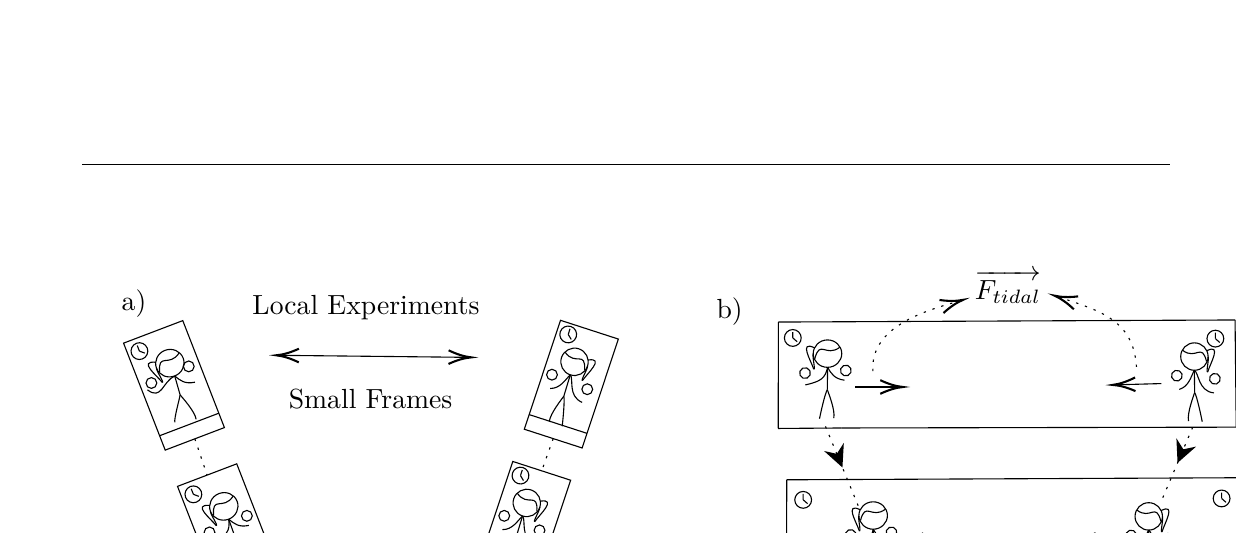
\begin{tikzpicture}[x=0.75pt,y=0.75pt,yscale=-1,xscale=1]
%uncomment if require: \path (0,236.2142791748047); %set diagram left start at 0, and has height of 236.2142791748047

%Shape: Ellipse [id:dp8845619089918026] 
\draw   (221.97,42.93) .. controls (223.09,39.46) and (226.82,37.56) .. (230.29,38.69) .. controls (233.76,39.81) and (235.66,43.53) .. (234.53,47) .. controls (233.41,50.47) and (229.68,52.37) .. (226.21,51.25) .. controls (222.75,50.12) and (220.85,46.4) .. (221.97,42.93) -- cycle ;
%Straight Lines [id:da5922373449905136] 
\draw    (226.21,51.25) -- (223.1,61.52) ;
%Curve Lines [id:da02567916525852243] 
\draw    (223.1,61.52) .. controls (222.29,62.68) and (216.48,69.91) .. (216.12,73.7) ;
%Curve Lines [id:da7587398678055812] 
\draw    (223.1,61.52) .. controls (223.61,63.98) and (222.56,73.9) .. (222.32,75.99) ;
%Curve Lines [id:da22598361850444237] 
\draw    (226.21,51.25) .. controls (227.96,53.24) and (224.9,61.5) .. (231.9,64.5) ;
%Curve Lines [id:da01286542074661634] 
\draw    (226.21,51.25) .. controls (223.72,53.6) and (221.5,57.83) .. (216.5,57.83) ;
%Curve Lines [id:da991021249040662] 
\draw    (223.77,40.39) .. controls (228.52,47.13) and (233.68,39.26) .. (233.11,49.05) ;
%Curve Lines [id:da20445642372859152] 
\draw    (234.82,44.1) .. controls (243.03,42.86) and (234.48,50.5) .. (232.03,54.04) ;
%Curve Lines [id:da10301266039412305] 
\draw    (232.03,54.04) .. controls (231.25,53.79) and (234.6,48.46) .. (234.53,47) ;
%Shape: Polygon [id:ds7930415743259898] 
\draw   (221.5,24.97) -- (249.37,34.01) -- (231.93,86.48) -- (204.06,77.45) -- cycle ;
%Straight Lines [id:da40505453521111856] 
\draw    (206.35,70.38) -- (234.22,79.42) ;
%Shape: Ellipse [id:dp5537243045215847] 
\draw   (39.7,43.17) .. controls (38.41,39.76) and (34.48,38.1) .. (30.93,39.45) .. controls (27.38,40.8) and (25.55,44.66) .. (26.85,48.06) .. controls (28.14,51.47) and (32.07,53.14) .. (35.62,51.79) .. controls (39.17,50.44) and (41,46.58) .. (39.7,43.17) -- cycle ;
%Straight Lines [id:da94570470992862] 
\draw    (35.62,51.79) -- (38.24,60.89) ;
%Curve Lines [id:da9915832886491431] 
\draw    (38.24,60.89) .. controls (39.12,62.01) and (45.42,68.89) .. (45.94,72.66) ;
%Curve Lines [id:da19847348195432746] 
\draw    (38.24,60.89) .. controls (37.81,63.39) and (35.34,72.06) .. (35.67,74.14) ;
%Curve Lines [id:da03339788672004884] 
\draw    (35.62,51.79) .. controls (29.5,54.69) and (29.5,63.69) .. (22.5,58.5) ;
%Curve Lines [id:da2662590138688341] 
\draw    (35.62,51.79) .. controls (38.3,53.99) and (40.5,55.83) .. (45.39,54.78) ;
%Curve Lines [id:da7457469637960004] 
\draw    (37.74,40.73) .. controls (33.07,47.81) and (27.44,40.24) .. (28.4,50.03) ;
%Curve Lines [id:da022279739126443987] 
\draw    (26.44,45.17) .. controls (17.88,44.45) and (27.03,51.56) .. (29.7,54.96) ;
%Curve Lines [id:da5752896257238964] 
\draw    (29.7,54.96) .. controls (30.51,54.66) and (26.83,49.53) .. (26.85,48.06) ;
%Shape: Polygon [id:ds2905274464619316] 
\draw   (39.51,25.12) -- (10.98,35.98) -- (31.05,87.51) -- (59.57,76.65) -- cycle ;
%Straight Lines [id:da20454095931660765] 
\draw    (56.93,69.71) -- (28.4,80.57) ;
%Shape: Ellipse [id:dp5640337384983714] 
\draw   (14.84,41.25) .. controls (14.05,39.17) and (15.1,36.83) .. (17.18,36.04) .. controls (19.27,35.24) and (21.6,36.29) .. (22.4,38.38) .. controls (23.19,40.46) and (22.14,42.8) .. (20.06,43.59) .. controls (17.97,44.39) and (15.64,43.34) .. (14.84,41.25) -- cycle ;
%Straight Lines [id:da26481603456137703] 
\draw    (17.58,37.15) -- (18.62,39.81) ;
%Straight Lines [id:da7429950747664196] 
\draw    (19.23,40.62) ;
%Straight Lines [id:da12626038383485017] 
\draw    (18.62,39.81) -- (21.25,40.79) ;
%Shape: Ellipse [id:dp9864227040089346] 
\draw   (221.37,30.54) .. controls (222.06,28.41) and (224.34,27.25) .. (226.46,27.94) .. controls (228.59,28.63) and (229.75,30.91) .. (229.06,33.03) .. controls (228.37,35.15) and (226.09,36.32) .. (223.97,35.63) .. controls (221.85,34.94) and (220.68,32.66) .. (221.37,30.54) -- cycle ;
%Straight Lines [id:da43338688563145156] 
\draw    (226.08,29.06) -- (225.22,31.78) ;
%Straight Lines [id:da6646590495130549] 
\draw    (225.19,32.79) ;
%Straight Lines [id:da16715025069300204] 
\draw    (225.22,31.78) -- (226.66,34.19) ;
%Shape: Circle [id:dp9848937377337077] 
\draw   (39.79,47.18) .. controls (39.79,45.74) and (40.95,44.57) .. (42.39,44.57) .. controls (43.83,44.57) and (45,45.74) .. (45,47.18) .. controls (45,48.62) and (43.83,49.78) .. (42.39,49.78) .. controls (40.95,49.78) and (39.79,48.62) .. (39.79,47.18) -- cycle ;
%Shape: Circle [id:dp21535919690002214] 
\draw   (214.79,51.18) .. controls (214.79,49.74) and (215.95,48.57) .. (217.39,48.57) .. controls (218.83,48.57) and (220,49.74) .. (220,51.18) .. controls (220,52.62) and (218.83,53.78) .. (217.39,53.78) .. controls (215.95,53.78) and (214.79,52.62) .. (214.79,51.18) -- cycle ;
%Straight Lines [id:da3252523654443955] 
\draw    (86.5,41.85) -- (176.5,42.81) ;
\draw [shift={(178.5,42.83)}, rotate = 180.61] [color={rgb, 255:red, 0; green, 0; blue, 0 }  ][line width=0.75]    (10.93,-3.29) .. controls (6.95,-1.4) and (3.31,-0.3) .. (0,0) .. controls (3.31,0.3) and (6.95,1.4) .. (10.93,3.29)   ;
\draw [shift={(84.5,41.83)}, rotate = 0.61] [color={rgb, 255:red, 0; green, 0; blue, 0 }  ][line width=0.75]    (10.93,-3.29) .. controls (6.95,-1.4) and (3.31,-0.3) .. (0,0) .. controls (3.31,0.3) and (6.95,1.4) .. (10.93,3.29)   ;
%Shape: Circle [id:dp08268945724087606] 
\draw   (21.79,55.18) .. controls (21.79,53.74) and (22.95,52.57) .. (24.39,52.57) .. controls (25.83,52.57) and (27,53.74) .. (27,55.18) .. controls (27,56.62) and (25.83,57.78) .. (24.39,57.78) .. controls (22.95,57.78) and (21.79,56.62) .. (21.79,55.18) -- cycle ;
%Shape: Circle [id:dp6268374799125749] 
\draw   (231.79,58.18) .. controls (231.79,56.74) and (232.95,55.57) .. (234.39,55.57) .. controls (235.83,55.57) and (237,56.74) .. (237,58.18) .. controls (237,59.62) and (235.83,60.78) .. (234.39,60.78) .. controls (232.95,60.78) and (231.79,59.62) .. (231.79,58.18) -- cycle ;
%Shape: Ellipse [id:dp715809346373786] 
\draw   (65.7,112.17) .. controls (64.41,108.76) and (60.48,107.1) .. (56.93,108.45) .. controls (53.38,109.8) and (51.55,113.66) .. (52.85,117.06) .. controls (54.14,120.47) and (58.07,122.14) .. (61.62,120.79) .. controls (65.17,119.44) and (67,115.58) .. (65.7,112.17) -- cycle ;
%Straight Lines [id:da13441255185162615] 
\draw    (61.62,120.79) -- (65.24,130.89) ;
%Curve Lines [id:da2843376237970534] 
\draw    (65.24,130.89) .. controls (66.12,132.01) and (72.42,138.89) .. (72.94,142.66) ;
%Curve Lines [id:da3312251858471662] 
\draw    (65.24,130.89) .. controls (64.81,133.39) and (66.27,143.28) .. (66.6,145.37) ;
%Curve Lines [id:da6956702089338089] 
\draw    (61.62,120.79) .. controls (62.5,126.5) and (60.5,128.5) .. (54.5,132.5) ;
%Curve Lines [id:da749436300726535] 
\draw    (61.62,120.79) .. controls (64.3,122.99) and (66.5,124.83) .. (71.39,123.78) ;
%Curve Lines [id:da6525342067470947] 
\draw    (63.74,109.73) .. controls (59.07,116.81) and (53.44,109.24) .. (54.4,119.03) ;
%Curve Lines [id:da5635297934423185] 
\draw    (52.44,114.17) .. controls (43.88,113.45) and (53.03,120.56) .. (55.7,123.96) ;
%Curve Lines [id:da501346911811827] 
\draw    (55.7,123.96) .. controls (56.51,123.66) and (52.83,118.53) .. (52.85,117.06) ;
%Shape: Polygon [id:ds18867780283835645] 
\draw   (65.51,94.12) -- (36.98,104.98) -- (57.05,156.51) -- (85.57,145.65) -- cycle ;
%Straight Lines [id:da48998031647798745] 
\draw    (82.93,138.71) -- (54.4,149.57) ;
%Shape: Ellipse [id:dp6656230572917436] 
\draw   (40.84,110.25) .. controls (40.05,108.17) and (41.1,105.83) .. (43.18,105.04) .. controls (45.27,104.24) and (47.6,105.29) .. (48.4,107.38) .. controls (49.19,109.46) and (48.14,111.8) .. (46.06,112.59) .. controls (43.97,113.39) and (41.64,112.34) .. (40.84,110.25) -- cycle ;
%Straight Lines [id:da16093826211414353] 
\draw    (43.58,106.15) -- (44.62,108.81) ;
%Straight Lines [id:da7440144108304729] 
\draw    (45.23,109.62) ;
%Straight Lines [id:da7316199746269114] 
\draw    (44.62,108.81) -- (47.25,109.79) ;
%Shape: Circle [id:dp9127272277050287] 
\draw   (67.79,119.18) .. controls (67.79,117.74) and (68.95,116.57) .. (70.39,116.57) .. controls (71.83,116.57) and (73,117.74) .. (73,119.18) .. controls (73,120.62) and (71.83,121.78) .. (70.39,121.78) .. controls (68.95,121.78) and (67.79,120.62) .. (67.79,119.18) -- cycle ;
%Shape: Circle [id:dp2498140842962333] 
\draw   (49.79,127.18) .. controls (49.79,125.74) and (50.95,124.57) .. (52.39,124.57) .. controls (53.83,124.57) and (55,125.74) .. (55,127.18) .. controls (55,128.62) and (53.83,129.78) .. (52.39,129.78) .. controls (50.95,129.78) and (49.79,128.62) .. (49.79,127.18) -- cycle ;
%Shape: Ellipse [id:dp2658036436486313] 
\draw   (198.97,110.93) .. controls (200.09,107.46) and (203.82,105.56) .. (207.29,106.69) .. controls (210.76,107.81) and (212.66,111.53) .. (211.53,115) .. controls (210.41,118.47) and (206.68,120.37) .. (203.21,119.25) .. controls (199.75,118.12) and (197.85,114.4) .. (198.97,110.93) -- cycle ;
%Straight Lines [id:da8719014696775342] 
\draw    (203.21,119.25) -- (200.1,129.52) ;
%Curve Lines [id:da051570842996915944] 
\draw    (200.1,129.52) .. controls (199.29,130.68) and (193.48,137.91) .. (193.12,141.7) ;
%Curve Lines [id:da8819966557451906] 
\draw    (200.1,129.52) .. controls (200.61,131.98) and (199.56,141.9) .. (199.32,143.99) ;
%Curve Lines [id:da9491659542651063] 
\draw    (203.21,119.25) .. controls (204.96,121.24) and (201.9,129.5) .. (208.9,132.5) ;
%Curve Lines [id:da825910538596563] 
\draw    (203.21,119.25) .. controls (200.72,121.6) and (198.5,125.83) .. (193.5,125.83) ;
%Curve Lines [id:da9638339091026531] 
\draw    (200.77,108.39) .. controls (205.52,115.13) and (210.68,107.26) .. (210.11,117.05) ;
%Curve Lines [id:da3218360504556874] 
\draw    (211.82,112.1) .. controls (220.03,110.86) and (211.48,118.5) .. (209.03,122.04) ;
%Curve Lines [id:da6066588459428122] 
\draw    (209.03,122.04) .. controls (208.25,121.79) and (211.6,116.46) .. (211.53,115) ;
%Shape: Polygon [id:ds6272366539284842] 
\draw   (198.5,92.97) -- (226.37,102.01) -- (208.93,154.48) -- (181.06,145.45) -- cycle ;
%Straight Lines [id:da7582971590133043] 
\draw    (183.35,138.38) -- (211.22,147.42) ;
%Shape: Ellipse [id:dp9989822451279453] 
\draw   (198.37,98.54) .. controls (199.06,96.41) and (201.34,95.25) .. (203.46,95.94) .. controls (205.59,96.63) and (206.75,98.91) .. (206.06,101.03) .. controls (205.37,103.15) and (203.09,104.32) .. (200.97,103.63) .. controls (198.85,102.94) and (197.68,100.66) .. (198.37,98.54) -- cycle ;
%Straight Lines [id:da6516055592456811] 
\draw    (203.08,97.06) -- (202.22,99.78) ;
%Straight Lines [id:da10537961289963804] 
\draw    (202.19,100.79) ;
%Straight Lines [id:da7003573251412809] 
\draw    (202.22,99.78) -- (203.66,102.19) ;
%Shape: Circle [id:dp9153257924520581] 
\draw   (191.79,119.18) .. controls (191.79,117.74) and (192.95,116.57) .. (194.39,116.57) .. controls (195.83,116.57) and (197,117.74) .. (197,119.18) .. controls (197,120.62) and (195.83,121.78) .. (194.39,121.78) .. controls (192.95,121.78) and (191.79,120.62) .. (191.79,119.18) -- cycle ;
%Shape: Circle [id:dp7190812682052716] 
\draw   (208.79,126.18) .. controls (208.79,124.74) and (209.95,123.57) .. (211.39,123.57) .. controls (212.83,123.57) and (214,124.74) .. (214,126.18) .. controls (214,127.62) and (212.83,128.78) .. (211.39,128.78) .. controls (209.95,128.78) and (208.79,127.62) .. (208.79,126.18) -- cycle ;
%Straight Lines [id:da6559882115862026] 
\draw  [dash pattern={on 0.84pt off 2.51pt}]  (45.31,82.08) -- (51.24,99.55) ;
%Straight Lines [id:da09428811438586093] 
\draw  [dash pattern={on 0.84pt off 2.51pt}]  (71.31,151.08) -- (80.5,174.83) ;
\draw [shift={(75.9,162.96)}, rotate = 248.85] [fill={rgb, 255:red, 0; green, 0; blue, 0 }  ][line width=0.08]  [draw opacity=0] (8.93,-4.29) -- (0,0) -- (8.93,4.29) -- cycle    ;
%Straight Lines [id:da32928167820138166] 
\draw  [dash pattern={on 0.84pt off 2.51pt}]  (217.99,81.97) -- (212.44,97.49) ;
%Straight Lines [id:da25813294131819386] 
\draw  [dash pattern={on 0.84pt off 2.51pt}]  (194.99,149.97) -- (186.5,173.83) ;
\draw [shift={(190.75,161.9)}, rotate = 289.59000000000003] [fill={rgb, 255:red, 0; green, 0; blue, 0 }  ][line width=0.08]  [draw opacity=0] (8.93,-4.29) -- (0,0) -- (8.93,4.29) -- cycle    ;
%Curve Lines [id:da9558862312300334] 
\draw    (4.59,224.78) .. controls (81.5,138.93) and (197.5,151.93) .. (263.68,222.89) ;
%Shape: Ellipse [id:dp4421283648946428] 
\draw   (520.31,42.41) .. controls (520.33,38.76) and (523.3,35.82) .. (526.94,35.84) .. controls (530.59,35.86) and (533.53,38.83) .. (533.51,42.47) .. controls (533.5,46.12) and (530.52,49.06) .. (526.88,49.04) .. controls (523.23,49.03) and (520.29,46.05) .. (520.31,42.41) -- cycle ;
%Straight Lines [id:da09543773566545144] 
\draw    (526.88,49.04) -- (527.03,59.77) ;
%Curve Lines [id:da9310169849029337] 
\draw    (527.03,59.77) .. controls (526.61,61.13) and (523.27,69.78) .. (524.08,73.5) ;
%Curve Lines [id:da029334180864113657] 
\draw    (527.03,59.77) .. controls (528.26,61.96) and (530.27,71.74) .. (530.68,73.8) ;
%Curve Lines [id:da536629125806277] 
\draw    (526.88,49.04) .. controls (529.14,50.41) and (528.74,59.21) .. (536.32,59.94) ;
%Curve Lines [id:da7498425473879569] 
\draw    (526.88,49.04) .. controls (525.21,52.04) and (524.39,56.75) .. (519.62,58.27) ;
%Curve Lines [id:da6157462202040205] 
\draw    (521.25,39.44) .. controls (527.83,44.42) and (530.35,35.35) .. (532.78,44.86) ;
%Curve Lines [id:da9246090421931514] 
\draw    (532.91,39.62) .. controls (540.35,35.94) and (534.53,45.81) .. (533.27,49.94) ;
%Curve Lines [id:da21440533173491572] 
\draw    (533.27,49.94) .. controls (532.44,49.93) and (534.02,43.84) .. (533.51,42.47) ;
%Straight Lines [id:da8237630169353887] 
\draw    (356.9,76.85) -- (547.06,76.45) ;
%Shape: Ellipse [id:dp6816906083883099] 
\draw   (357.01,40.97) .. controls (356.98,37.32) and (353.88,34.39) .. (350.08,34.42) .. controls (346.28,34.45) and (343.23,37.43) .. (343.25,41.07) .. controls (343.28,44.72) and (346.38,47.65) .. (350.18,47.63) .. controls (353.98,47.6) and (357.04,44.62) .. (357.01,40.97) -- cycle ;
%Straight Lines [id:da7325459457524279] 
\draw    (350.18,47.63) -- (350.05,58.36) ;
%Curve Lines [id:da4487369544422213] 
\draw    (350.05,58.36) .. controls (350.49,59.71) and (353.99,68.35) .. (353.16,72.07) ;
%Curve Lines [id:da8270208960740166] 
\draw    (350.05,58.36) .. controls (348.77,60.55) and (346.7,70.33) .. (346.28,72.4) ;
%Curve Lines [id:da5268682421202648] 
\draw    (350.18,47.63) .. controls (349.01,53.28) and (346.44,54.46) .. (339.42,56.12) ;
%Curve Lines [id:da8777722792318512] 
\draw    (350.18,47.63) .. controls (351.92,50.62) and (353.34,53.12) .. (358.29,53.84) ;
%Curve Lines [id:da05328552981032897] 
\draw    (356.02,38) .. controls (349.18,43) and (346.53,33.95) .. (344.02,43.46) ;
%Curve Lines [id:da2548428383536683] 
\draw    (343.88,38.22) .. controls (336.11,34.56) and (342.2,44.42) .. (343.52,48.54) ;
%Curve Lines [id:da6154358168503964] 
\draw    (343.52,48.54) .. controls (344.38,48.53) and (342.73,42.44) .. (343.25,41.07) ;
%Straight Lines [id:da18542050746244865] 
\draw    (356.9,76.85) -- (326.38,77.08) ;
%Straight Lines [id:da7437595187763801] 
\draw    (335.71,36.44) ;
%Shape: Ellipse [id:dp3213557914507905] 
\draw   (532.97,33.78) .. controls (532.98,31.55) and (534.8,29.75) .. (537.04,29.76) .. controls (539.27,29.77) and (541.07,31.59) .. (541.06,33.82) .. controls (541.05,36.05) and (539.23,37.85) .. (537,37.84) .. controls (534.76,37.83) and (532.96,36.01) .. (532.97,33.78) -- cycle ;
%Straight Lines [id:da44306178265708684] 
\draw    (537.01,30.94) -- (537.02,33.8) ;
%Straight Lines [id:da9836391028510754] 
\draw    (537.3,34.77) ;
%Straight Lines [id:da7299858556428198] 
\draw    (537.02,33.8) -- (539.12,35.66) ;
%Shape: Circle [id:dp8374137390910636] 
\draw   (356.52,48.26) .. controls (357.02,46.91) and (358.52,46.23) .. (359.87,46.73) .. controls (361.22,47.23) and (361.9,48.73) .. (361.4,50.08) .. controls (360.9,51.43) and (359.4,52.12) .. (358.05,51.61) .. controls (356.7,51.11) and (356.02,49.61) .. (356.52,48.26) -- cycle ;
%Shape: Circle [id:dp6239004075600636] 
\draw   (515.97,52.45) .. controls (515.53,51.08) and (516.29,49.61) .. (517.66,49.17) .. controls (519.03,48.74) and (520.5,49.49) .. (520.93,50.86) .. controls (521.37,52.24) and (520.61,53.7) .. (519.24,54.14) .. controls (517.87,54.58) and (516.4,53.82) .. (515.97,52.45) -- cycle ;
%Shape: Circle [id:dp42397620033944095] 
\draw   (336.86,49.49) .. controls (337.36,48.14) and (338.86,47.45) .. (340.21,47.95) .. controls (341.56,48.45) and (342.24,49.95) .. (341.74,51.3) .. controls (341.24,52.65) and (339.74,53.34) .. (338.39,52.84) .. controls (337.04,52.34) and (336.36,50.84) .. (336.86,49.49) -- cycle ;
%Shape: Circle [id:dp9618512415431733] 
\draw   (534.29,53.95) .. controls (533.85,52.58) and (534.61,51.12) .. (535.98,50.68) .. controls (537.35,50.24) and (538.82,51) .. (539.26,52.37) .. controls (539.69,53.74) and (538.94,55.21) .. (537.56,55.64) .. controls (536.19,56.08) and (534.73,55.32) .. (534.29,53.95) -- cycle ;
%Shape: Ellipse [id:dp5971363794232412] 
\draw   (498.31,119.41) .. controls (498.33,115.76) and (501.3,112.82) .. (504.94,112.84) .. controls (508.59,112.86) and (511.53,115.83) .. (511.51,119.47) .. controls (511.5,123.12) and (508.52,126.06) .. (504.88,126.04) .. controls (501.23,126.03) and (498.29,123.05) .. (498.31,119.41) -- cycle ;
%Straight Lines [id:da8652938247648636] 
\draw    (504.88,126.04) -- (505.03,136.77) ;
%Curve Lines [id:da17539982950467814] 
\draw    (505.03,136.77) .. controls (504.61,138.13) and (501.27,146.78) .. (502.08,150.5) ;
%Curve Lines [id:da4138532395424208] 
\draw    (505.03,136.77) .. controls (506.26,138.96) and (508.27,148.74) .. (508.68,150.8) ;
%Curve Lines [id:da7184793888503163] 
\draw    (504.88,126.04) .. controls (507.14,127.41) and (506.74,136.21) .. (514.32,136.94) ;
%Curve Lines [id:da675200277367431] 
\draw    (504.88,126.04) .. controls (503.21,129.04) and (502.39,133.75) .. (497.62,135.27) ;
%Curve Lines [id:da3616115188436895] 
\draw    (499.25,116.44) .. controls (505.83,121.42) and (508.35,112.35) .. (510.78,121.86) ;
%Curve Lines [id:da43346376658244434] 
\draw    (510.91,116.62) .. controls (518.35,112.94) and (512.53,122.81) .. (511.27,126.94) ;
%Curve Lines [id:da06079032920027938] 
\draw    (511.27,126.94) .. controls (510.44,126.93) and (512.02,120.84) .. (511.51,119.47) ;
%Straight Lines [id:da22871820440554758] 
\draw    (360.9,152.85) -- (551.06,152.45) ;
%Shape: Ellipse [id:dp8189266792751762] 
\draw   (379.01,118.97) .. controls (378.98,115.32) and (375.88,112.39) .. (372.08,112.42) .. controls (368.28,112.45) and (365.23,115.43) .. (365.25,119.07) .. controls (365.28,122.72) and (368.38,125.65) .. (372.18,125.63) .. controls (375.98,125.6) and (379.04,122.62) .. (379.01,118.97) -- cycle ;
%Straight Lines [id:da885626797361388] 
\draw    (372.18,125.63) -- (372.05,136.36) ;
%Curve Lines [id:da17120326720531653] 
\draw    (372.05,136.36) .. controls (372.49,137.71) and (375.99,146.35) .. (375.16,150.07) ;
%Curve Lines [id:da8569549406138941] 
\draw    (372.05,136.36) .. controls (370.77,138.55) and (368.7,148.33) .. (368.28,150.4) ;
%Curve Lines [id:da5997524751501591] 
\draw    (372.18,125.63) .. controls (371.01,131.28) and (368.44,132.46) .. (361.42,134.12) ;
%Curve Lines [id:da09100238496427715] 
\draw    (372.18,125.63) .. controls (373.92,128.62) and (375.34,131.12) .. (380.29,131.84) ;
%Curve Lines [id:da5387076172818799] 
\draw    (378.02,116) .. controls (371.18,121) and (368.53,111.95) .. (366.02,121.46) ;
%Curve Lines [id:da279800635300691] 
\draw    (365.88,116.22) .. controls (358.11,112.56) and (364.2,122.42) .. (365.52,126.54) ;
%Curve Lines [id:da12844013360274653] 
\draw    (365.52,126.54) .. controls (366.38,126.53) and (364.73,120.44) .. (365.25,119.07) ;
%Straight Lines [id:da7845865113684638] 
\draw    (360.9,152.85) -- (330.38,153.08) ;
%Shape: Ellipse [id:dp4906589489555522] 
\draw   (334.37,111.5) .. controls (334.36,109.27) and (336.15,107.45) .. (338.39,107.43) .. controls (340.62,107.42) and (342.44,109.21) .. (342.46,111.44) .. controls (342.48,113.68) and (340.68,115.5) .. (338.45,115.52) .. controls (336.21,115.53) and (334.39,113.74) .. (334.37,111.5) -- cycle ;
%Straight Lines [id:da11373134346717673] 
\draw    (338.37,108.61) -- (338.42,111.47) ;
%Straight Lines [id:da47916210916584157] 
\draw    (338.71,112.44) ;
%Straight Lines [id:da14071157746865115] 
\draw    (338.42,111.47) -- (340.55,113.31) ;
%Shape: Ellipse [id:dp800219484817623] 
\draw   (535.97,110.78) .. controls (535.98,108.55) and (537.8,106.75) .. (540.04,106.76) .. controls (542.27,106.77) and (544.07,108.59) .. (544.06,110.82) .. controls (544.05,113.05) and (542.23,114.85) .. (540,114.84) .. controls (537.76,114.83) and (535.96,113.01) .. (535.97,110.78) -- cycle ;
%Straight Lines [id:da41619306911405096] 
\draw    (540.01,107.94) -- (540.02,110.8) ;
%Straight Lines [id:da46704159013612445] 
\draw    (540.3,111.77) ;
%Straight Lines [id:da35200360744658155] 
\draw    (540.02,110.8) -- (542.12,112.66) ;
%Shape: Circle [id:dp9439363312725977] 
\draw   (378.52,126.26) .. controls (379.02,124.91) and (380.52,124.23) .. (381.87,124.73) .. controls (383.22,125.23) and (383.9,126.73) .. (383.4,128.08) .. controls (382.9,129.43) and (381.4,130.12) .. (380.05,129.61) .. controls (378.7,129.11) and (378.02,127.61) .. (378.52,126.26) -- cycle ;
%Shape: Circle [id:dp5819859799311946] 
\draw   (493.97,129.45) .. controls (493.53,128.08) and (494.29,126.61) .. (495.66,126.17) .. controls (497.03,125.74) and (498.5,126.49) .. (498.93,127.86) .. controls (499.37,129.24) and (498.61,130.7) .. (497.24,131.14) .. controls (495.87,131.58) and (494.4,130.82) .. (493.97,129.45) -- cycle ;
%Shape: Circle [id:dp7500155742053494] 
\draw   (358.86,127.49) .. controls (359.36,126.14) and (360.86,125.45) .. (362.21,125.95) .. controls (363.56,126.45) and (364.24,127.95) .. (363.74,129.3) .. controls (363.24,130.65) and (361.74,131.34) .. (360.39,130.84) .. controls (359.04,130.34) and (358.36,128.84) .. (358.86,127.49) -- cycle ;
%Shape: Circle [id:dp6827709647881515] 
\draw   (512.29,130.95) .. controls (511.85,129.58) and (512.61,128.12) .. (513.98,127.68) .. controls (515.35,127.24) and (516.82,128) .. (517.26,129.37) .. controls (517.69,130.74) and (516.94,132.21) .. (515.56,132.64) .. controls (514.19,133.08) and (512.73,132.32) .. (512.29,130.95) -- cycle ;
%Straight Lines [id:da9530274407929566] 
\draw    (330.5,101.81) -- (330.38,153.08) ;
%Straight Lines [id:da616699308541967] 
\draw    (550.5,100.81) -- (551.06,152.45) ;
%Straight Lines [id:da13925293728193133] 
\draw    (330.5,101.81) -- (550.5,100.81) ;
%Straight Lines [id:da738885523463638] 
\draw    (326.5,25.81) -- (326.38,77.08) ;
%Straight Lines [id:da10639804868906544] 
\draw    (546.5,24.81) -- (547.06,76.45) ;
%Straight Lines [id:da4325374107027895] 
\draw    (326.5,25.81) -- (546.5,24.81) ;
%Straight Lines [id:da9134538901817384] 
\draw    (363.5,57.1) -- (384.5,57.1) ;
\draw [shift={(386.5,57.1)}, rotate = 180] [color={rgb, 255:red, 0; green, 0; blue, 0 }  ][line width=0.75]    (10.93,-3.29) .. controls (6.95,-1.4) and (3.31,-0.3) .. (0,0) .. controls (3.31,0.3) and (6.95,1.4) .. (10.93,3.29)   ;
%Straight Lines [id:da9209098129688724] 
\draw    (510.97,55.45) -- (489.5,56.05) ;
\draw [shift={(487.5,56.1)}, rotate = 358.4] [color={rgb, 255:red, 0; green, 0; blue, 0 }  ][line width=0.75]    (10.93,-3.29) .. controls (6.95,-1.4) and (3.31,-0.3) .. (0,0) .. controls (3.31,0.3) and (6.95,1.4) .. (10.93,3.29)   ;
%Curve Lines [id:da18681909786348094] 
\draw  [dash pattern={on 0.84pt off 2.51pt}]  (372,49.43) .. controls (370.57,27.15) and (399.69,19.77) .. (413.63,15.66) ;
\draw [shift={(415.5,15.1)}, rotate = 522.9] [color={rgb, 255:red, 0; green, 0; blue, 0 }  ][line width=0.75]    (10.93,-3.29) .. controls (6.95,-1.4) and (3.31,-0.3) .. (0,0) .. controls (3.31,0.3) and (6.95,1.4) .. (10.93,3.29)   ;
%Curve Lines [id:da14593266010418837] 
\draw  [dash pattern={on 0.84pt off 2.51pt}]  (499,47.43) .. controls (497.55,24.8) and (481.51,20.36) .. (461.38,13.73) ;
\draw [shift={(459.5,13.1)}, rotate = 378.43] [color={rgb, 255:red, 0; green, 0; blue, 0 }  ][line width=0.75]    (10.93,-3.29) .. controls (6.95,-1.4) and (3.31,-0.3) .. (0,0) .. controls (3.31,0.3) and (6.95,1.4) .. (10.93,3.29)   ;
%Straight Lines [id:da48022203911277606] 
\draw    (386.5,131.1) -- (404.5,130.71) ;
\draw [shift={(406.5,130.67)}, rotate = 538.77] [color={rgb, 255:red, 0; green, 0; blue, 0 }  ][line width=0.75]    (10.93,-3.29) .. controls (6.95,-1.4) and (3.31,-0.3) .. (0,0) .. controls (3.31,0.3) and (6.95,1.4) .. (10.93,3.29)   ;
%Straight Lines [id:da030843895076588357] 
\draw    (491.97,130.45) -- (470.5,131.05) ;
\draw [shift={(468.5,131.1)}, rotate = 358.4] [color={rgb, 255:red, 0; green, 0; blue, 0 }  ][line width=0.75]    (10.93,-3.29) .. controls (6.95,-1.4) and (3.31,-0.3) .. (0,0) .. controls (3.31,0.3) and (6.95,1.4) .. (10.93,3.29)   ;
%Curve Lines [id:da5900875227624809] 
\draw    (313.59,226.21) .. controls (390.5,140.36) and (506.5,153.36) .. (572.68,224.32) ;
%Straight Lines [id:da737020393963671] 
\draw  [dash pattern={on 0.84pt off 2.51pt}]  (349.16,76.07) -- (365.5,115.72) ;
\draw [shift={(357.33,95.89)}, rotate = 247.6] [fill={rgb, 255:red, 0; green, 0; blue, 0 }  ][line width=0.08]  [draw opacity=0] (10.72,-5.15) -- (0,0) -- (10.72,5.15) -- (7.12,0) -- cycle    ;
%Straight Lines [id:da623172367069025] 
\draw  [dash pattern={on 0.84pt off 2.51pt}]  (526.08,76.5) -- (511.5,110.86) ;
\draw [shift={(518.79,93.68)}, rotate = 292.99] [fill={rgb, 255:red, 0; green, 0; blue, 0 }  ][line width=0.08]  [draw opacity=0] (10.72,-5.15) -- (0,0) -- (10.72,5.15) -- (7.12,0) -- cycle    ;
%Shape: Ellipse [id:dp4848379340166973] 
\draw   (329.37,33.5) .. controls (329.36,31.27) and (331.15,29.45) .. (333.39,29.43) .. controls (335.62,29.42) and (337.44,31.21) .. (337.46,33.44) .. controls (337.48,35.68) and (335.68,37.5) .. (333.45,37.52) .. controls (331.21,37.53) and (329.39,35.74) .. (329.37,33.5) -- cycle ;
%Straight Lines [id:da3621711428879839] 
\draw    (333.37,30.61) -- (333.42,33.47) ;
%Straight Lines [id:da6763317966334057] 
\draw    (333.71,34.44) ;
%Straight Lines [id:da357058133676478] 
\draw    (333.42,33.47) -- (335.55,35.31) ;

% Text Node
\draw (130,18.83) node   [align=left] {Local Experiments };
% Text Node
\draw (130,62.83) node   [align=left] {Small Frames};
% Text Node
\draw (437,9.1) node    {$\overrightarrow{F_{tidal}}$};
% Text Node
\draw (442,193.67) node   [align=left] {"Large" Frames};
% Text Node
\draw (16,17) node   [align=left] {a)};
% Text Node
\draw (303,21) node   [align=left] {b)};


\end{tikzpicture}

\caption{The Strong Equivalence Principle states that \textbf{all physics} must be the same locally for two free falling observers. However, observers in a "large" non-local reference frame such as this will be able to detect a gravitational field by noticing the tidal forces between objects.}
\label{fig:my_label}
\end{figure}

\pagebreak


\section{Doppler Effects under acceleration \& Gravity}

Normally, in the case of Special Relativity we understand the concept of Doppler shifting. If the receiver has a different velocity when compared to the source, they will detect a different wavelength.

\begin{figure}[h!]
\centering


\tikzset{every picture/.style={line width=0.75pt}} %set default line width to 0.75pt        

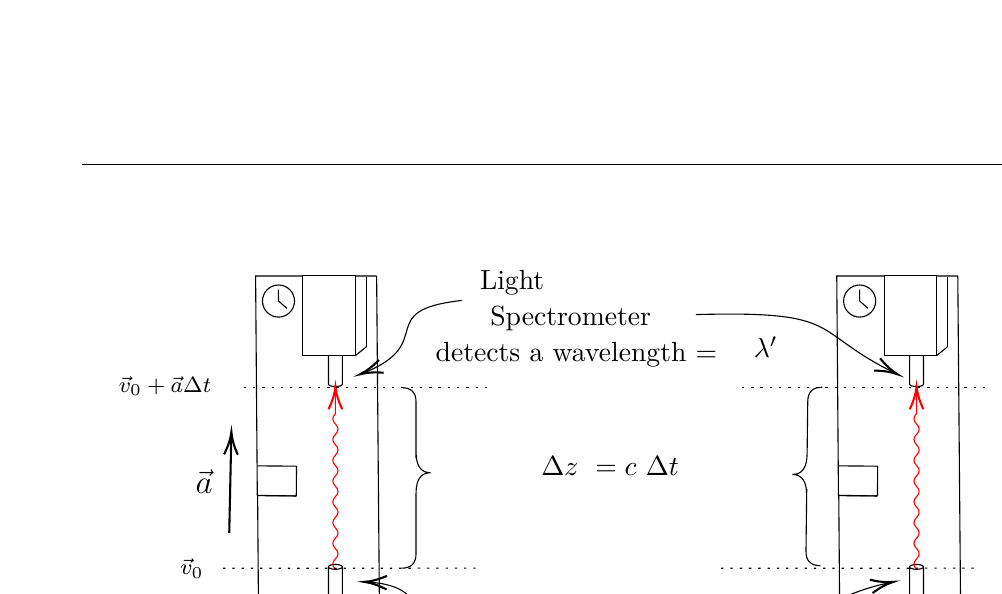
\begin{tikzpicture}[x=0.75pt,y=0.75pt,yscale=-1,xscale=1]
%uncomment if require: \path (0,331.921875); %set diagram left start at 0, and has height of 331.921875

%Shape: Can [id:dp7652948660117864] 
\draw   (116,49.95) -- (116,68.91) .. controls (116,69.55) and (114.5,70.08) .. (112.65,70.08) .. controls (110.8,70.08) and (109.3,69.55) .. (109.3,68.91) -- (109.3,49.95) .. controls (109.3,49.3) and (110.8,48.78) .. (112.65,48.78) .. controls (114.5,48.78) and (116,49.3) .. (116,49.95) .. controls (116,50.6) and (114.5,51.12) .. (112.65,51.12) .. controls (110.8,51.12) and (109.3,50.6) .. (109.3,49.95) ;
%Straight Lines [id:da47427135870330317] 
\draw [line width=0.75]    (61.5,140.6) -- (62.49,93.89) ;
\draw [shift={(62.54,91.89)}, rotate = 451.22] [color={rgb, 255:red, 0; green, 0; blue, 0 }  ][line width=0.75]    (10.93,-3.29) .. controls (6.95,-1.4) and (3.31,-0.3) .. (0,0) .. controls (3.31,0.3) and (6.95,1.4) .. (10.93,3.29)   ;
%Straight Lines [id:da8588567612763613] 
\draw    (93.8,122.79) -- (75.17,122.62) -- (75.99,228.27) -- (134.3,228.27) ;
%Straight Lines [id:da5737995741736945] 
\draw    (134.3,214.08) -- (75.99,214.08) ;
%Curve Lines [id:da285481691447776] 
\draw    (100.63,228.79) .. controls (94.06,234.84) and (95.7,246.67) .. (98.99,254.02) ;
%Curve Lines [id:da17111562949052517] 
\draw    (110.48,228.01) .. controls (120.34,233.53) and (116.23,245.09) .. (112.13,254.81) ;
%Straight Lines [id:da608181235108741] 
\draw    (112.13,254.81) -- (110.48,239.57) ;
%Straight Lines [id:da9574700917062451] 
\draw    (105.72,268.9) -- (110.48,239.57) ;
%Straight Lines [id:da7983792586303715] 
\draw    (98.99,254.02) -- (102.27,241.15) ;
%Straight Lines [id:da2949986993249043] 
\draw    (105.72,268.9) -- (102.27,241.15) ;
%Straight Lines [id:da4906969044706222] 
\draw    (86.75,136.52) ;
%Straight Lines [id:da513010416947036] 
\draw    (132.51,16.83) -- (74.2,16.83) -- (75.02,122.48) -- (93.8,122.79) ;
%Straight Lines [id:da2641449484941776] 
\draw    (93.91,108.42) -- (75.02,108.29) ;
%Shape: Ellipse [id:dp7594531786749046] 
\draw   (77.51,28.87) .. controls (77.51,24.61) and (80.97,21.15) .. (85.23,21.15) .. controls (89.5,21.15) and (92.95,24.61) .. (92.95,28.87) .. controls (92.95,33.14) and (89.5,36.6) .. (85.23,36.6) .. controls (80.97,36.6) and (77.51,33.14) .. (77.51,28.87) -- cycle ;
%Straight Lines [id:da38423358074561387] 
\draw    (85.18,23.41) -- (85.23,28.87) ;
%Straight Lines [id:da5886538282592515] 
\draw    (85.78,30.72) ;
%Straight Lines [id:da47901088665670155] 
\draw    (85.23,28.87) -- (89.27,32.4) ;
%Straight Lines [id:da83045176136826] 
\draw    (132.51,16.83) -- (134.3,228.27) ;
%Straight Lines [id:da806087253711919] 
\draw    (93.91,108.42) -- (93.8,122.79) ;
%Shape: Cube [id:dp27833093906588724] 
\draw  [fill={rgb, 255:red, 255; green, 255; blue, 255 }  ,fill opacity=1 ] (97,179.38) -- (102.3,174.08) -- (127.5,174.08) -- (127.5,213.77) -- (122.2,219.08) -- (97,219.08) -- cycle ; \draw   (127.5,174.08) -- (122.2,179.38) -- (97,179.38) ; \draw   (122.2,179.38) -- (122.2,219.08) ;
%Shape: Can [id:dp8499494754338972] 
\draw  [fill={rgb, 255:red, 255; green, 255; blue, 255 }  ,fill opacity=1 ] (116,156.95) -- (116,175.91) .. controls (116,176.55) and (114.5,177.08) .. (112.65,177.08) .. controls (110.8,177.08) and (109.3,176.55) .. (109.3,175.91) -- (109.3,156.95) .. controls (109.3,156.3) and (110.8,155.78) .. (112.65,155.78) .. controls (114.5,155.78) and (116,156.3) .. (116,156.95) .. controls (116,157.6) and (114.5,158.12) .. (112.65,158.12) .. controls (110.8,158.12) and (109.3,157.6) .. (109.3,156.95) ;
%Straight Lines [id:da13156339819342433] 
\draw    (127.5,17.26) -- (127.5,50.95) ;
%Straight Lines [id:da039499447469547366] 
\draw    (122.2,55.26) -- (127.5,50.95) ;
%Shape: Rectangle [id:dp7313328547958049] 
\draw  [fill={rgb, 255:red, 255; green, 255; blue, 255 }  ,fill opacity=1 ] (97,16.57) -- (122.2,16.57) -- (122.2,55.26) -- (97,55.26) -- cycle ;
%Curve Lines [id:da6606310196138308] 
\draw    (179.5,225.58) .. controls (124.06,222.61) and (181.33,167.3) .. (128.15,164.25) ;
\draw [shift={(126.5,164.17)}, rotate = 362.05] [color={rgb, 255:red, 0; green, 0; blue, 0 }  ][line width=0.75]    (10.93,-3.29) .. controls (6.95,-1.4) and (3.31,-0.3) .. (0,0) .. controls (3.31,0.3) and (6.95,1.4) .. (10.93,3.29)   ;
%Curve Lines [id:da30512768738610463] 
\draw    (173.5,28.58) .. controls (130.16,33.5) and (162.5,49.1) .. (126.21,63.52) ;
\draw [shift={(124.5,64.17)}, rotate = 339.48] [color={rgb, 255:red, 0; green, 0; blue, 0 }  ][line width=0.75]    (10.93,-3.29) .. controls (6.95,-1.4) and (3.31,-0.3) .. (0,0) .. controls (3.31,0.3) and (6.95,1.4) .. (10.93,3.29)   ;
%Straight Lines [id:da8499830370849735] 
\draw [color={rgb, 255:red, 255; green, 0; blue, 0 }  ,draw opacity=1 ]   (112.65,158.12) .. controls (110.98,156.45) and (110.98,154.79) .. (112.65,153.12) .. controls (114.32,151.45) and (114.32,149.79) .. (112.65,148.12) .. controls (110.98,146.45) and (110.98,144.79) .. (112.65,143.12) .. controls (114.32,141.45) and (114.32,139.79) .. (112.65,138.12) .. controls (110.98,136.45) and (110.98,134.79) .. (112.65,133.12) .. controls (114.32,131.45) and (114.32,129.79) .. (112.65,128.12) .. controls (110.98,126.45) and (110.98,124.79) .. (112.65,123.12) .. controls (114.32,121.45) and (114.32,119.79) .. (112.65,118.12) .. controls (110.98,116.45) and (110.98,114.79) .. (112.65,113.12) .. controls (114.32,111.45) and (114.32,109.79) .. (112.65,108.12) .. controls (110.98,106.45) and (110.98,104.79) .. (112.65,103.12) .. controls (114.32,101.45) and (114.32,99.79) .. (112.65,98.12) .. controls (110.98,96.45) and (110.98,94.79) .. (112.65,93.12) .. controls (114.32,91.45) and (114.32,89.79) .. (112.65,88.12) .. controls (110.98,86.45) and (110.98,84.79) .. (112.65,83.12) -- (112.65,80.08) -- (112.65,72.08) ;
\draw [shift={(112.65,70.08)}, rotate = 450] [color={rgb, 255:red, 255; green, 0; blue, 0 }  ,draw opacity=1 ][line width=0.75]    (10.93,-3.29) .. controls (6.95,-1.4) and (3.31,-0.3) .. (0,0) .. controls (3.31,0.3) and (6.95,1.4) .. (10.93,3.29)   ;
%Shape: Brace [id:dp5594199305245107] 
\draw   (144.5,157.58) .. controls (149.17,157.58) and (151.5,155.25) .. (151.5,150.58) -- (151.5,121.58) .. controls (151.5,114.91) and (153.83,111.58) .. (158.5,111.58) .. controls (153.83,111.58) and (151.5,108.25) .. (151.5,101.58)(151.5,104.58) -- (151.5,77.58) .. controls (151.5,72.91) and (149.17,70.58) .. (144.5,70.58) ;
%Straight Lines [id:da7970954928059399] 
\draw  [dash pattern={on 0.84pt off 2.51pt}]  (68.5,70.58) -- (185.5,70.58) ;
%Straight Lines [id:da783868655451514] 
\draw  [dash pattern={on 0.84pt off 2.51pt}]  (58.5,157.6) -- (183.5,157.58) ;
%Shape: Can [id:dp8552091246342881] 
\draw   (396,49.95) -- (396,68.91) .. controls (396,69.55) and (394.5,70.08) .. (392.65,70.08) .. controls (390.8,70.08) and (389.3,69.55) .. (389.3,68.91) -- (389.3,49.95) .. controls (389.3,49.3) and (390.8,48.78) .. (392.65,48.78) .. controls (394.5,48.78) and (396,49.3) .. (396,49.95) .. controls (396,50.6) and (394.5,51.12) .. (392.65,51.12) .. controls (390.8,51.12) and (389.3,50.6) .. (389.3,49.95) ;
%Straight Lines [id:da01777645408026851] 
\draw    (373.8,122.79) -- (355.17,122.62) -- (355.99,228.27) -- (414.3,228.27) ;
%Straight Lines [id:da9094445960130315] 
\draw    (414.3,214.08) -- (355.99,214.08) ;
%Straight Lines [id:da6406485027325557] 
\draw    (366.75,136.52) ;
%Straight Lines [id:da9512018910577791] 
\draw    (412.51,16.83) -- (354.2,16.83) -- (355.02,122.48) -- (373.8,122.79) ;
%Straight Lines [id:da3255268357860086] 
\draw    (373.91,108.42) -- (355.02,108.29) ;
%Shape: Ellipse [id:dp6259036068498025] 
\draw   (357.51,28.87) .. controls (357.51,24.61) and (360.97,21.15) .. (365.23,21.15) .. controls (369.5,21.15) and (372.95,24.61) .. (372.95,28.87) .. controls (372.95,33.14) and (369.5,36.6) .. (365.23,36.6) .. controls (360.97,36.6) and (357.51,33.14) .. (357.51,28.87) -- cycle ;
%Straight Lines [id:da7441130043312898] 
\draw    (365.18,23.41) -- (365.23,28.87) ;
%Straight Lines [id:da4682509198797593] 
\draw    (365.78,30.72) ;
%Straight Lines [id:da5602884622313555] 
\draw    (365.23,28.87) -- (369.27,32.4) ;
%Straight Lines [id:da9091881590150592] 
\draw    (412.51,16.83) -- (414.3,228.27) ;
%Straight Lines [id:da1901518511629654] 
\draw    (373.91,108.42) -- (373.8,122.79) ;
%Shape: Cube [id:dp3377983039624415] 
\draw  [fill={rgb, 255:red, 255; green, 255; blue, 255 }  ,fill opacity=1 ] (377,179.38) -- (382.3,174.08) -- (407.5,174.08) -- (407.5,213.77) -- (402.2,219.08) -- (377,219.08) -- cycle ; \draw   (407.5,174.08) -- (402.2,179.38) -- (377,179.38) ; \draw   (402.2,179.38) -- (402.2,219.08) ;
%Shape: Can [id:dp6424557876961308] 
\draw  [fill={rgb, 255:red, 255; green, 255; blue, 255 }  ,fill opacity=1 ] (396,156.95) -- (396,175.91) .. controls (396,176.55) and (394.5,177.08) .. (392.65,177.08) .. controls (390.8,177.08) and (389.3,176.55) .. (389.3,175.91) -- (389.3,156.95) .. controls (389.3,156.3) and (390.8,155.78) .. (392.65,155.78) .. controls (394.5,155.78) and (396,156.3) .. (396,156.95) .. controls (396,157.6) and (394.5,158.12) .. (392.65,158.12) .. controls (390.8,158.12) and (389.3,157.6) .. (389.3,156.95) ;
%Straight Lines [id:da03443586587440173] 
\draw    (407.5,17.26) -- (407.5,50.95) ;
%Straight Lines [id:da5384404833609466] 
\draw    (402.2,55.26) -- (407.5,50.95) ;
%Shape: Rectangle [id:dp0008233195153486417] 
\draw  [fill={rgb, 255:red, 255; green, 255; blue, 255 }  ,fill opacity=1 ] (377,16.57) -- (402.2,16.57) -- (402.2,55.26) -- (377,55.26) -- cycle ;
%Curve Lines [id:da02862579315575875] 
\draw    (286.3,222.4) .. controls (357.94,225.38) and (306.82,179.86) .. (380.38,164.41) ;
\draw [shift={(381.5,164.17)}, rotate = 528.55] [color={rgb, 255:red, 0; green, 0; blue, 0 }  ][line width=0.75]    (10.93,-3.29) .. controls (6.95,-1.4) and (3.31,-0.3) .. (0,0) .. controls (3.31,0.3) and (6.95,1.4) .. (10.93,3.29)   ;
%Curve Lines [id:da0980081700088502] 
\draw    (286.3,35.4) .. controls (358.57,33.42) and (340.67,43.2) .. (382.22,63.55) ;
\draw [shift={(383.5,64.17)}, rotate = 205.68] [color={rgb, 255:red, 0; green, 0; blue, 0 }  ][line width=0.75]    (10.93,-3.29) .. controls (6.95,-1.4) and (3.31,-0.3) .. (0,0) .. controls (3.31,0.3) and (6.95,1.4) .. (10.93,3.29)   ;
%Straight Lines [id:da2992984442349256] 
\draw [color={rgb, 255:red, 255; green, 0; blue, 0 }  ,draw opacity=1 ]   (392.65,158.12) .. controls (390.98,156.45) and (390.98,154.79) .. (392.65,153.12) .. controls (394.32,151.45) and (394.32,149.79) .. (392.65,148.12) .. controls (390.98,146.45) and (390.98,144.79) .. (392.65,143.12) .. controls (394.32,141.45) and (394.32,139.79) .. (392.65,138.12) .. controls (390.98,136.45) and (390.98,134.79) .. (392.65,133.12) .. controls (394.32,131.45) and (394.32,129.79) .. (392.65,128.12) .. controls (390.98,126.45) and (390.98,124.79) .. (392.65,123.12) .. controls (394.32,121.45) and (394.32,119.79) .. (392.65,118.12) .. controls (390.98,116.45) and (390.98,114.79) .. (392.65,113.12) .. controls (394.32,111.45) and (394.32,109.79) .. (392.65,108.12) .. controls (390.98,106.45) and (390.98,104.79) .. (392.65,103.12) .. controls (394.32,101.45) and (394.32,99.79) .. (392.65,98.12) .. controls (390.98,96.45) and (390.98,94.79) .. (392.65,93.12) .. controls (394.32,91.45) and (394.32,89.79) .. (392.65,88.12) .. controls (390.98,86.45) and (390.98,84.79) .. (392.65,83.12) -- (392.65,80.08) -- (392.65,72.08) ;
\draw [shift={(392.65,70.08)}, rotate = 450] [color={rgb, 255:red, 255; green, 0; blue, 0 }  ,draw opacity=1 ][line width=0.75]    (10.93,-3.29) .. controls (6.95,-1.4) and (3.31,-0.3) .. (0,0) .. controls (3.31,0.3) and (6.95,1.4) .. (10.93,3.29)   ;
%Shape: Brace [id:dp06527009850176135] 
\draw   (347.3,70.4) .. controls (342.63,70.35) and (340.27,72.65) .. (340.22,77.32) -- (339.92,102.5) .. controls (339.85,109.17) and (337.48,112.47) .. (332.81,112.42) .. controls (337.48,112.47) and (339.77,115.83) .. (339.69,122.5)(339.73,119.5) -- (339.38,149.32) .. controls (339.32,153.99) and (341.62,156.35) .. (346.29,156.4) ;
%Straight Lines [id:da07232872335467722] 
\draw  [dash pattern={on 0.84pt off 2.51pt}]  (308.5,70.58) -- (425.5,70.58) ;
%Straight Lines [id:da9679390145382802] 
\draw  [dash pattern={on 0.84pt off 2.51pt}]  (298.5,157.6) -- (423.5,157.58) ;
%Straight Lines [id:da24299802534685555] 
\draw [line width=0.75]    (441.5,100.6) -- (441.31,143.4) ;
\draw [shift={(441.3,145.4)}, rotate = 270.26] [color={rgb, 255:red, 0; green, 0; blue, 0 }  ][line width=0.75]    (10.93,-3.29) .. controls (6.95,-1.4) and (3.31,-0.3) .. (0,0) .. controls (3.31,0.3) and (6.95,1.4) .. (10.93,3.29)   ;

% Text Node
\draw (49.36,115.83) node  [font=\large]  {$\vec{a}$};
% Text Node
\draw (231,218.17) node   [align=left] {Light Source};
% Text Node
\draw (200,20.17) node   [align=left] {Light };
% Text Node
\draw (226,37.4) node   [align=left] {Spectrometer};
% Text Node
\draw (231,54.58) node   [align=left] {detects a wavelength = };
% Text Node
\draw (245,108.26) node    {$\Delta z\ =c\ \Delta t$};
% Text Node
\draw (230,237.17) node   [align=left] {Produces wavelength = };
% Text Node
\draw (319,234.08) node    {$\lambda $};
% Text Node
\draw (320,51.08) node    {$\lambda ^{\prime }$};
% Text Node
\draw (32.5,69.76) node  [font=\footnotesize]  {$\vec{v}_{0} +\vec{a} \Delta t\ $};
% Text Node
\draw (43.5,157.76) node  [font=\footnotesize]  {$\vec{v}_{0}$};
% Text Node
\draw (451.36,115.83) node  [font=\large]  {$\vec{g}$};


\end{tikzpicture}

\caption{The Strong Equivalence Principle states that \textbf{all physics} must be the same locally for these two observers}
\label{fig:my_label}
\end{figure}

Consider an accelerating frame given in Figure 3. With a light source producing light of wavelength $\lambda$ and a receiver a distance $\Delta z$ apart. By the time the light covers that distance, the velocity of the receiver will have increased by $\Delta v = a \Delta t$. A higher velocity would imply that they will detect the light at a lower wavelength $\lambda^{\prime}$. We can calculate the shift:

\begin{equation}
\label{Frequency Change Discrete}
    \frac{\Delta{\lambda}}{\lambda_0} = \frac{\lambda^{\prime}-\lambda}{\lambda} = \frac{\Delta v}{c} = \frac{a \Delta z}{c^3}
\end{equation}

Now we can invoke the Strong Equivalence Principle, and assert that a stationary observer in a gravitational field should see exactly the same effect: a light ray going against gravity will be detected at a lower frequency at a larger height. In fact we may get a more mathematically exact form. If we break $\Delta z$ into infinitesimal chunks and add the frequency red-shift over small local frames along a path, we find:

\begin{equation}
\label{Frequency Change continuous}
    \frac{d\lambda}{\lambda} = -\frac{\vec{g}\cdot \vec{dr}}{c^3} 
\end{equation}

 Now we will integrate this equation. We will find, to first order \sn{One actually integrates and gets $\frac{\lambda^{\prime}}{\lambda_0} = \exp{\frac{\Delta \Phi}{c^3}} \approx 1 + \frac{\Delta \Phi}{c^3}$}:

\begin{equation}
\label{Frequency Change continuous}
    \frac{\Delta{\lambda}}{\lambda_0} = -\frac{1}{c^3} \int_{z_0}^{z_0 + \Delta z} (-\vec{\nabla}\Phi) \cdot \vec{dS}  =  \frac{\Delta\Phi}{c^3}
\end{equation}

This is the amount of gravitational redshift. Observers in higher potentials (i.e. further away from gravitational sources), see light produced from lower potentials as "red-er" \sn{lower frequency / higher wavelength} than normal. Hence, we have seen a straightforward prediction of the Strong Equivalence Principle.   
\\
\pagebreak


\part{Manifolds}
Now we have a postulate that allows us to do physics in local, free falling frames, can we piece it together some how to get some sort of picture of physics in large global frames? The answer is yes!  It turns out that this framework of piecing together local reference frames into a greater whole, is basically the study of manifolds. This begins our mathematical excursion into differential geometry. 

\section{What is a Manifold?}

An $n$-dimensional Manifold is simply a space that locally looks like $\mathbb{R}^n$. Informally speaking, if you zoom in really close to the Manifold, on a fine-grained level, it \textit{looks like} a flat patch of an $n$-dimensional flat space, $\mathbb{R}^n$. What exactly we mean by \textit{"looks like"} will be formalised later on.

For now, consider an example of a $2$-dimensional manifold: the surface of a sphere, also called $\mathbb{S}^2$. Looking at it's round shape, one would conclude it looks nothing like $\mathbb{R}^n$, but if you take a point and zoom in enough (like in Figure 4), the space around it looks pretty much flat --- so much so that it looks like $\mathbb{R}^2$

%\begin{comment}
\begin{figure}[h!]
\centering


\tikzset{every picture/.style={line width=0.75pt}} %set default line width to 0.75pt        

\begin{tikzpicture}[x=0.75pt,y=0.75pt,yscale=-0.75,xscale=0.75]
%uncomment if require: \path (0,300); %set diagram left start at 0, and has height of 300

%Shape: Circle [id:dp14136974738901475] 
\draw  [line width=1.5]  (59,145.25) .. controls (59,89.33) and (104.33,44) .. (160.25,44) .. controls (216.17,44) and (261.5,89.33) .. (261.5,145.25) .. controls (261.5,201.17) and (216.17,246.5) .. (160.25,246.5) .. controls (104.33,246.5) and (59,201.17) .. (59,145.25) -- cycle ;
%Curve Lines [id:da24823790568944393] 
\draw    (160.25,44) .. controls (75.5,89.7) and (93.5,200.7) .. (127.5,239.5) ;
%Curve Lines [id:da5198328458496135] 
\draw    (160.25,44) .. controls (202.5,40) and (257.5,148.7) .. (196.5,240.7) ;
%Curve Lines [id:da3707324968485255] 
\draw    (160.25,44) .. controls (177.5,67.7) and (202.5,147.7) .. (169.5,247.7) ;
%Curve Lines [id:da800009697742498] 
\draw    (160.25,44) .. controls (132.5,73.5) and (131.5,209.5) .. (151.5,247.5) ;
%Curve Lines [id:da4720591674101946] 
\draw    (59,145.25) .. controls (89.5,165) and (214.5,166) .. (261.5,145.25) ;
%Curve Lines [id:da47184546195959] 
\draw    (69.5,101) .. controls (112.5,111) and (205.5,117) .. (247.5,96) ;
%Curve Lines [id:da09121697192437872] 
\draw    (72.5,193) .. controls (115.5,203) and (178.5,215) .. (250.5,193) ;
%Curve Lines [id:da6989591203767807] 
\draw    (92.5,72) .. controls (135.5,82) and (191.5,85) .. (229.5,71) ;
%Shape: Rectangle [id:dp25904253699597457] 
\draw  [fill={rgb, 255:red, 255; green, 255; blue, 255 }  ,fill opacity=1 ] (208.84,102.75) -- (219.33,102.39) -- (223.66,113.25) -- (213.17,113.61) -- cycle ;
%Curve Lines [id:da4787165657296577] 
\draw    (224,107) .. controls (302.11,85.75) and (384.67,90.59) .. (451.49,199.99) ;
\draw [shift={(452.5,201.64)}, rotate = 238.88] [color={rgb, 255:red, 0; green, 0; blue, 0 }  ][line width=0.75]    (10.93,-3.29) .. controls (6.95,-1.4) and (3.31,-0.3) .. (0,0) .. controls (3.31,0.3) and (6.95,1.4) .. (10.93,3.29)   ;
%Shape: Rectangle [id:dp7247614884184055] 
\draw   (499.38,206.04) -- (568.46,217.32) -- (440.62,236.96) -- (371.54,225.68) -- cycle ;
%Straight Lines [id:da19252000285981596] 
\draw    (530.5,211.5) -- (406.5,230.5) ;
%Straight Lines [id:da9408515383339116] 
\draw    (510.5,225.5) -- (441.5,214.5) ;

% Text Node
\draw (163,266) node  [font=\Large]  {$\mathbb{S}^{2}$};
% Text Node
\draw (473,195) node  [font=\Large]   {$\mathbb{R}^{2}$};


\end{tikzpicture}

\caption{$\mathbb{S}^2$ looks locally like $\mathbb{R}^2$}
\label{fig:my_label}
\end{figure}
%\end{comment}




Some other examples of Manifolds are given in Figure 4. 



\section{Building up the Mathematical toolbox}

We first begin with the definition of a map from a set $M$ to a set $N$. These sets could be the set of all points in some space, or could even be some other abstract sets.\\


%\begin{sidebox}[Def: Map]
%Given two sets $M = \{m_1,m_2,m_3 ...\}$ and $N = \{n_1,n_2,n_3 ...\}$ we can define a \textbf{map} $\phi$ denoted $\phi: M \rightarrow N$, such that every element in $M$ is assigned to only one element in $N$. 
%\end{sidebox}

\begin{tcolorbox}
\textbf{Definition: Map} \\ \\ Given two sets $M = \{m_1,m_2,m_3 ...\}$ and $N = \{n_1,n_2,n_3 ...\}$ we can define a \textbf{map} $\phi$ denoted $\phi: M \rightarrow N$, such that every element in $M$ is assigned to only one element in $N$. 
\end{tcolorbox}

%\begin{comment}
\begin{figure}[h!]
\centering


\tikzset{every picture/.style={line width=0.75pt}} %set default line width to 0.75pt        

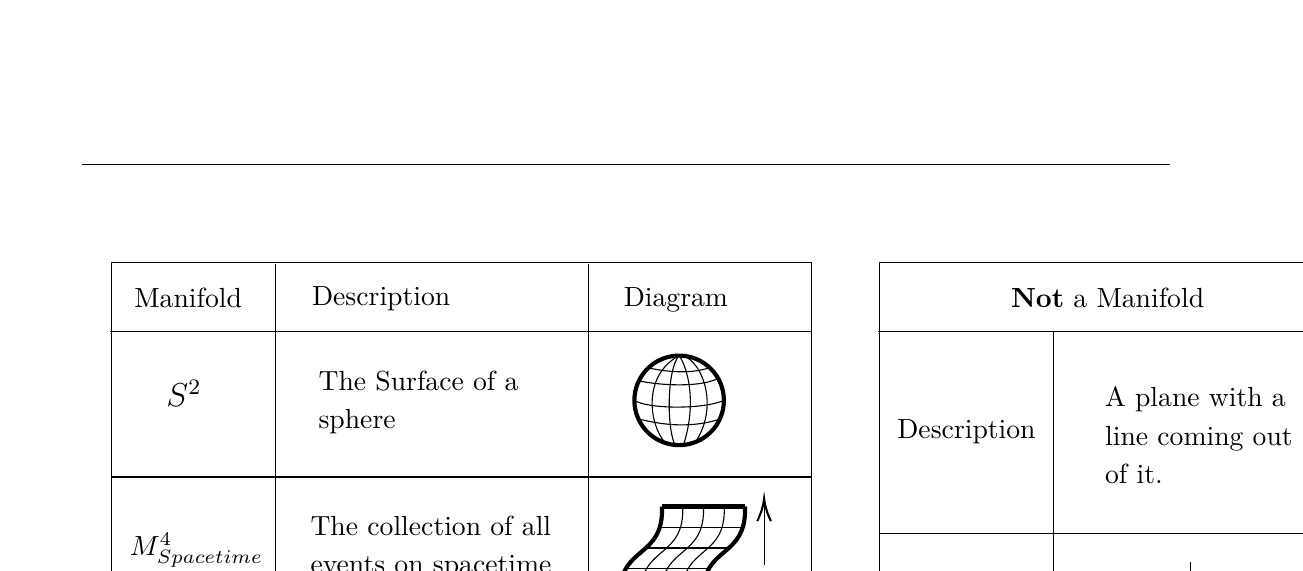
\begin{tikzpicture}[x=0.75pt,y=0.75pt,yscale=-1,xscale=1]
%uncomment if require: \path (0,300); %set diagram left start at 0, and has height of 300

%Shape: Rectangle [id:dp5055672709450891] 
\draw   (10,23.25) -- (347.5,23.25) -- (347.5,269.81) -- (10,269.81) -- cycle ;
%Straight Lines [id:da0541799082187675] 
\draw    (89,24.25) -- (89,271.04) ;
%Straight Lines [id:da23352752150023814] 
\draw    (240,24.25) -- (240,271.04) ;
%Straight Lines [id:da06548087685456694] 
\draw    (9.5,56.81) -- (347.5,56.81) ;
%Straight Lines [id:da18517670886629478] 
\draw    (10.5,126.81) -- (347.5,126.81) ;
%Shape: Ellipse [id:dp7952388603476075] 
\draw  [line width=1.5]  (262,89.88) .. controls (262,77.97) and (271.65,68.31) .. (283.56,68.31) .. controls (295.47,68.31) and (305.13,77.97) .. (305.13,89.88) .. controls (305.13,101.79) and (295.47,111.44) .. (283.56,111.44) .. controls (271.65,111.44) and (262,101.79) .. (262,89.88) -- cycle ;
%Curve Lines [id:da05410223871968256] 
\draw    (283.56,68.31) .. controls (265.51,78.05) and (269.35,101.69) .. (276.59,109.95) ;
%Curve Lines [id:da3455245039536605] 
\draw    (283.56,68.31) .. controls (292.56,67.46) and (304.28,90.61) .. (291.29,110.21) ;
%Curve Lines [id:da9189647133107459] 
\draw    (283.56,68.31) .. controls (287.24,73.36) and (292.56,90.4) .. (285.54,111.7) ;
%Curve Lines [id:da4481132931593548] 
\draw    (283.56,68.31) .. controls (277.65,74.6) and (277.44,103.56) .. (281.7,111.66) ;
%Curve Lines [id:da38300192168922753] 
\draw    (262,89.88) .. controls (268.5,94.09) and (295.12,94.3) .. (305.13,89.88) ;
%Curve Lines [id:da38137977621584307] 
\draw    (264.24,80.45) .. controls (273.39,82.58) and (293.2,83.86) .. (302.15,79.39) ;
%Curve Lines [id:da04890609493928899] 
\draw    (264.88,99.05) .. controls (274.03,101.18) and (287.45,103.74) .. (302.79,99.05) ;
%Curve Lines [id:da04149727882873311] 
\draw    (269.14,74.28) .. controls (278.29,76.41) and (290.22,77.05) .. (298.31,74.07) ;
%Straight Lines [id:da29473496999817406] 
\draw    (10.5,196.81) -- (347.5,196.81) ;
%Curve Lines [id:da5439437877543751] 
\draw [line width=1.5]    (255.3,182.01) .. controls (255.3,160.01) and (276.3,166.01) .. (275.3,141.01) ;
%Curve Lines [id:da255440401061676] 
\draw [line width=1.5]    (295.3,182.01) .. controls (295.3,160.01) and (316.3,166.01) .. (315.3,141.01) ;
%Curve Lines [id:da6650410265474336] 
\draw    (285.3,182.01) .. controls (285.3,160.01) and (306.3,166.01) .. (305.3,141.01) ;
%Curve Lines [id:da060471114907779455] 
\draw    (275.3,182.01) .. controls (275.3,160.01) and (296.3,166.01) .. (295.3,141.01) ;
%Curve Lines [id:da3258458726920288] 
\draw    (265.3,182.01) .. controls (265.3,160.01) and (286.3,166.01) .. (285.3,141.01) ;
%Straight Lines [id:da13841234614977682] 
\draw [line width=1.5]    (275.3,141.01) -- (315.3,141.01) ;
%Straight Lines [id:da18882901638612415] 
\draw    (274.3,151.01) -- (314.3,151.01) ;
%Straight Lines [id:da89050699232276] 
\draw    (267.3,161.01) -- (307.3,161.01) ;
%Straight Lines [id:da051472078505148344] 
\draw    (257.3,171.01) -- (297.3,171.01) ;
%Straight Lines [id:da31470130901111015] 
\draw [line width=1.5]    (255.3,182.01) -- (295.3,182.01) ;
%Shape: Grid [id:dp21296831699294327] 
\draw  [draw opacity=0] (262,213) -- (306,213) -- (306,257) -- (262,257) -- cycle ; \draw   (273,213) -- (273,257)(284,213) -- (284,257)(295,213) -- (295,257) ; \draw   (262,224) -- (306,224)(262,235) -- (306,235)(262,246) -- (306,246) ; \draw   (262,213) -- (306,213) -- (306,257) -- (262,257) -- cycle ;
%Straight Lines [id:da14482847924712283] 
\draw [line width=1.5]    (262,213) -- (262,257) ;
%Straight Lines [id:da9197709924047432] 
\draw [line width=1.5]    (306,213) -- (306,257) ;
%Straight Lines [id:da6116277026306363] 
\draw [line width=1.5]    (262,213) -- (306,213) ;
%Straight Lines [id:da9799718870426737] 
\draw [line width=1.5]    (262,257) -- (306,257) ;
%Straight Lines [id:da6129412013470565] 
\draw    (324.5,169.12) -- (324.5,139.12) ;
\draw [shift={(324.5,137.12)}, rotate = 450] [color={rgb, 255:red, 0; green, 0; blue, 0 }  ][line width=0.75]    (10.93,-3.29) .. controls (6.95,-1.4) and (3.31,-0.3) .. (0,0) .. controls (3.31,0.3) and (6.95,1.4) .. (10.93,3.29)   ;
%Shape: Rectangle [id:dp5618197350421079] 
\draw   (380,23.25) -- (610,23.25) -- (610,269.81) -- (380,269.81) -- cycle ;
%Straight Lines [id:da5603031935610843] 
\draw    (464,56.25) -- (464,271.04) ;
%Straight Lines [id:da3425453114657584] 
\draw    (610,24.25) -- (610,271.04) ;
%Straight Lines [id:da40207323347409885] 
\draw    (379.5,56.81) -- (609.5,56.81) ;
%Straight Lines [id:da22956656581506496] 
\draw    (380.5,153.81) -- (609.5,153.81) ;
%Straight Lines [id:da4705069650634177] 
%\draw [line width=1.5]    (676,213) -- (676,257) ;
%Straight Lines [id:da8219513759179924] 
%\draw    (694.5,169.12) -- (694.5,139.12) ;
%\draw [shift={(694.5,137.12)}, rotate = 450] [color={rgb, 255:red, 0; green, 0; blue, 0 }  ][line width=0.75]    (10.93,-3.29) .. controls (6.95,-1.4) and (3.31,-0.3) .. (0,0) .. controls (3.31,0.3) and (6.95,1.4) .. (10.93,3.29)   ;
%Shape: Grid [id:dp9150048565967743] 
\draw  [draw opacity=0] (526.27,201.1) -- (569.47,209.45) -- (533.03,236.02) -- (489.83,227.67) -- cycle ; \draw   (537.07,203.19) -- (500.63,229.76)(547.87,205.28) -- (511.43,231.85)(558.67,207.36) -- (522.23,233.93) ; \draw   (514.12,209.96) -- (557.32,218.31)(501.97,218.81) -- (545.18,227.17) ; \draw   (526.27,201.1) -- (569.47,209.45) -- (533.03,236.02) -- (489.83,227.67) -- cycle ;
%Straight Lines [id:da1662153638321211] 
\draw [line width=1.5]    (526.27,201.1) -- (488.76,228.45) ;
%Straight Lines [id:da013861031847801186] 
\draw [line width=1.5]    (569.47,209.45) -- (531.96,236.8) ;
%Straight Lines [id:da7960824830468722] 
\draw [line width=1.5]    (526.27,201.1) -- (569.47,209.45) ;
%Straight Lines [id:da7285367784814745] 
\draw [line width=1.5]    (488.76,228.45) -- (531.96,236.8) ;
%Straight Lines [id:da6055829475842325] 
\draw    (530,218.96) -- (530,168.96) -- (530,167.96) ;

% Text Node
\draw (47,40.41) node   [align=left] {Manifold};
% Text Node
\draw (140,40.81) node   [align=left] {Description};
% Text Node
\draw (158,90.81) node   [align=left] {The Surface of a \\sphere};
% Text Node
\draw (45,86.62) node  [font=\large]  {$S^{2}$};
% Text Node
\draw (51,162) node    {$M^{4}_{Spacetime}$};
% Text Node
\draw (164,161) node   [align=left] {The collection of all \\events on spacetime};
% Text Node
\draw (46,234.46) node    {$\mathbb{R}^{n}$};
% Text Node
\draw (164,233.46) node   [align=left] {The collection of all \\n-tuples of real\\numbers};
% Text Node
\draw (195,253.46) node  [font=\footnotesize]  {$( x_{1} ,x_{2} ,..,x_{n})$};
% Text Node
\draw (282,41.46) node   [align=left] {Diagram};
% Text Node
\draw (325,177.12) node   [align=left] {time};
% Text Node
\draw (422,104.81) node   [align=left] {Description};
% Text Node
\draw (534,106.81) node   [align=left] {A plane with a \\line coming out\\of it.};
% Text Node
\draw (490,40.41) node   [align=left] {\textbf{Not} a Manifold};
% Text Node
\draw (423,213.81) node   [align=left] {Diagram};

\end{tikzpicture}

\caption{Examples of manifolds, and one non-example}
\label{fig:my_label 2}
\end{figure}
%\end{comment}

It is fruitful to point out that each element in $M$ should be mapped to only one element in $N$ but it need not be a distinct element. This means that multiple elements in $M$ can map to the same element in $N$. 

\begin{figure}[h!]
\centering


\tikzset{every picture/.style={line width=0.75pt}} %set default line width to 0.75pt        

\begin{tikzpicture}[x=0.75pt,y=0.75pt,yscale=-1,xscale=1]
%uncomment if require: \path (0,138.64999389648438); %set diagram left start at 0, and has height of 138.64999389648438

%Shape: Ellipse [id:dp1420442812577336] 
\draw   (30.75,10) .. controls (38.9,10) and (45.5,32.25) .. (45.5,59.71) .. controls (45.5,87.16) and (38.9,109.41) .. (30.75,109.41) .. controls (22.6,109.41) and (16,87.16) .. (16,59.71) .. controls (16,32.25) and (22.6,10) .. (30.75,10) -- cycle ;
%Flowchart: Connector [id:dp8953212953940233] 
\draw   (25,28.91) .. controls (25,25.87) and (27.46,23.41) .. (30.5,23.41) .. controls (33.54,23.41) and (36,25.87) .. (36,28.91) .. controls (36,31.95) and (33.54,34.41) .. (30.5,34.41) .. controls (27.46,34.41) and (25,31.95) .. (25,28.91) -- cycle ;
%Flowchart: Connector [id:dp2848939032822819] 
\draw   (25,48.91) .. controls (25,45.87) and (27.46,43.41) .. (30.5,43.41) .. controls (33.54,43.41) and (36,45.87) .. (36,48.91) .. controls (36,51.95) and (33.54,54.41) .. (30.5,54.41) .. controls (27.46,54.41) and (25,51.95) .. (25,48.91) -- cycle ;
%Flowchart: Connector [id:dp5739620978835185] 
\draw   (25,68.91) .. controls (25,65.87) and (27.46,63.41) .. (30.5,63.41) .. controls (33.54,63.41) and (36,65.87) .. (36,68.91) .. controls (36,71.95) and (33.54,74.41) .. (30.5,74.41) .. controls (27.46,74.41) and (25,71.95) .. (25,68.91) -- cycle ;
%Flowchart: Connector [id:dp7333462920620866] 
\draw   (25,88.91) .. controls (25,85.87) and (27.46,83.41) .. (30.5,83.41) .. controls (33.54,83.41) and (36,85.87) .. (36,88.91) .. controls (36,91.95) and (33.54,94.41) .. (30.5,94.41) .. controls (27.46,94.41) and (25,91.95) .. (25,88.91) -- cycle ;
%Shape: Ellipse [id:dp08269242679614708] 
\draw   (110.75,10) .. controls (118.9,10) and (125.5,32.25) .. (125.5,59.71) .. controls (125.5,87.16) and (118.9,109.41) .. (110.75,109.41) .. controls (102.6,109.41) and (96,87.16) .. (96,59.71) .. controls (96,32.25) and (102.6,10) .. (110.75,10) -- cycle ;
%Flowchart: Connector [id:dp4549117443373931] 
\draw   (105,28.91) .. controls (105,25.87) and (107.46,23.41) .. (110.5,23.41) .. controls (113.54,23.41) and (116,25.87) .. (116,28.91) .. controls (116,31.95) and (113.54,34.41) .. (110.5,34.41) .. controls (107.46,34.41) and (105,31.95) .. (105,28.91) -- cycle ;
%Flowchart: Connector [id:dp8456860450689725] 
\draw   (105,48.91) .. controls (105,45.87) and (107.46,43.41) .. (110.5,43.41) .. controls (113.54,43.41) and (116,45.87) .. (116,48.91) .. controls (116,51.95) and (113.54,54.41) .. (110.5,54.41) .. controls (107.46,54.41) and (105,51.95) .. (105,48.91) -- cycle ;
%Flowchart: Connector [id:dp4548331314660914] 
\draw   (105,68.91) .. controls (105,65.87) and (107.46,63.41) .. (110.5,63.41) .. controls (113.54,63.41) and (116,65.87) .. (116,68.91) .. controls (116,71.95) and (113.54,74.41) .. (110.5,74.41) .. controls (107.46,74.41) and (105,71.95) .. (105,68.91) -- cycle ;
%Flowchart: Connector [id:dp9704140818144571] 
\draw   (105,88.91) .. controls (105,85.87) and (107.46,83.41) .. (110.5,83.41) .. controls (113.54,83.41) and (116,85.87) .. (116,88.91) .. controls (116,91.95) and (113.54,94.41) .. (110.5,94.41) .. controls (107.46,94.41) and (105,91.95) .. (105,88.91) -- cycle ;
%Shape: Ellipse [id:dp9581267181233748] 
\draw   (216.75,10) .. controls (224.9,10) and (231.5,32.25) .. (231.5,59.71) .. controls (231.5,87.16) and (224.9,109.41) .. (216.75,109.41) .. controls (208.6,109.41) and (202,87.16) .. (202,59.71) .. controls (202,32.25) and (208.6,10) .. (216.75,10) -- cycle ;
%Flowchart: Connector [id:dp6497865039955351] 
\draw   (211,28.91) .. controls (211,25.87) and (213.46,23.41) .. (216.5,23.41) .. controls (219.54,23.41) and (222,25.87) .. (222,28.91) .. controls (222,31.95) and (219.54,34.41) .. (216.5,34.41) .. controls (213.46,34.41) and (211,31.95) .. (211,28.91) -- cycle ;
%Flowchart: Connector [id:dp5223014418669796] 
\draw   (211,48.91) .. controls (211,45.87) and (213.46,43.41) .. (216.5,43.41) .. controls (219.54,43.41) and (222,45.87) .. (222,48.91) .. controls (222,51.95) and (219.54,54.41) .. (216.5,54.41) .. controls (213.46,54.41) and (211,51.95) .. (211,48.91) -- cycle ;
%Flowchart: Connector [id:dp9644782269162713] 
\draw   (211,68.91) .. controls (211,65.87) and (213.46,63.41) .. (216.5,63.41) .. controls (219.54,63.41) and (222,65.87) .. (222,68.91) .. controls (222,71.95) and (219.54,74.41) .. (216.5,74.41) .. controls (213.46,74.41) and (211,71.95) .. (211,68.91) -- cycle ;
%Flowchart: Connector [id:dp10343306192800705] 
\draw   (211,88.91) .. controls (211,85.87) and (213.46,83.41) .. (216.5,83.41) .. controls (219.54,83.41) and (222,85.87) .. (222,88.91) .. controls (222,91.95) and (219.54,94.41) .. (216.5,94.41) .. controls (213.46,94.41) and (211,91.95) .. (211,88.91) -- cycle ;
%Shape: Ellipse [id:dp5503163786841285] 
\draw   (296.75,10) .. controls (304.9,10) and (311.5,32.25) .. (311.5,59.71) .. controls (311.5,87.16) and (304.9,109.41) .. (296.75,109.41) .. controls (288.6,109.41) and (282,87.16) .. (282,59.71) .. controls (282,32.25) and (288.6,10) .. (296.75,10) -- cycle ;
%Flowchart: Connector [id:dp626120592849738] 
\draw   (291,28.91) .. controls (291,25.87) and (293.46,23.41) .. (296.5,23.41) .. controls (299.54,23.41) and (302,25.87) .. (302,28.91) .. controls (302,31.95) and (299.54,34.41) .. (296.5,34.41) .. controls (293.46,34.41) and (291,31.95) .. (291,28.91) -- cycle ;
%Flowchart: Connector [id:dp02098383473614618] 
\draw   (291,48.91) .. controls (291,45.87) and (293.46,43.41) .. (296.5,43.41) .. controls (299.54,43.41) and (302,45.87) .. (302,48.91) .. controls (302,51.95) and (299.54,54.41) .. (296.5,54.41) .. controls (293.46,54.41) and (291,51.95) .. (291,48.91) -- cycle ;
%Flowchart: Connector [id:dp5664884094502642] 
\draw   (291,68.91) .. controls (291,65.87) and (293.46,63.41) .. (296.5,63.41) .. controls (299.54,63.41) and (302,65.87) .. (302,68.91) .. controls (302,71.95) and (299.54,74.41) .. (296.5,74.41) .. controls (293.46,74.41) and (291,71.95) .. (291,68.91) -- cycle ;
%Flowchart: Connector [id:dp8291638196061419] 
\draw   (291,88.91) .. controls (291,85.87) and (293.46,83.41) .. (296.5,83.41) .. controls (299.54,83.41) and (302,85.87) .. (302,88.91) .. controls (302,91.95) and (299.54,94.41) .. (296.5,94.41) .. controls (293.46,94.41) and (291,91.95) .. (291,88.91) -- cycle ;
%Straight Lines [id:da06713382649662214] 
\draw    (30.5,28.91) -- (108.56,48.43) ;
\draw [shift={(110.5,48.91)}, rotate = 194.04] [color={rgb, 255:red, 0; green, 0; blue, 0 }  ][line width=0.75]    (10.93,-3.29) .. controls (6.95,-1.4) and (3.31,-0.3) .. (0,0) .. controls (3.31,0.3) and (6.95,1.4) .. (10.93,3.29)   ;
%Straight Lines [id:da8769750066355422] 
\draw    (30.5,48.91) -- (108.56,68.43) ;
\draw [shift={(110.5,68.91)}, rotate = 194.04] [color={rgb, 255:red, 0; green, 0; blue, 0 }  ][line width=0.75]    (10.93,-3.29) .. controls (6.95,-1.4) and (3.31,-0.3) .. (0,0) .. controls (3.31,0.3) and (6.95,1.4) .. (10.93,3.29)   ;
%Straight Lines [id:da5282651581840918] 
\draw    (30.5,88.91) -- (108.56,69.4) ;
\draw [shift={(110.5,68.91)}, rotate = 525.96] [color={rgb, 255:red, 0; green, 0; blue, 0 }  ][line width=0.75]    (10.93,-3.29) .. controls (6.95,-1.4) and (3.31,-0.3) .. (0,0) .. controls (3.31,0.3) and (6.95,1.4) .. (10.93,3.29)   ;
%Straight Lines [id:da8266039326319738] 
\draw    (30.5,68.91) -- (108.56,88.43) ;
\draw [shift={(110.5,88.91)}, rotate = 194.04] [color={rgb, 255:red, 0; green, 0; blue, 0 }  ][line width=0.75]    (10.93,-3.29) .. controls (6.95,-1.4) and (3.31,-0.3) .. (0,0) .. controls (3.31,0.3) and (6.95,1.4) .. (10.93,3.29)   ;
%Curve Lines [id:da34095628197655903] 
\draw [color={rgb, 255:red, 42; green, 120; blue, 19 }  ,draw opacity=1 ]   (138.75,52.71) .. controls (149.5,69.89) and (140.5,60.89) .. (168.5,42.89) ;
%Straight Lines [id:da7300337948761282] 
\draw    (216.5,88.91) -- (294.56,69.4) ;
\draw [shift={(296.5,68.91)}, rotate = 525.96] [color={rgb, 255:red, 0; green, 0; blue, 0 }  ][line width=0.75]    (10.93,-3.29) .. controls (6.95,-1.4) and (3.31,-0.3) .. (0,0) .. controls (3.31,0.3) and (6.95,1.4) .. (10.93,3.29)   ;
%Straight Lines [id:da6361761087179325] 
\draw    (216.75,29) -- (295.06,48.43) ;
\draw [shift={(297,48.91)}, rotate = 193.94] [color={rgb, 255:red, 0; green, 0; blue, 0 }  ][line width=0.75]    (10.93,-3.29) .. controls (6.95,-1.4) and (3.31,-0.3) .. (0,0) .. controls (3.31,0.3) and (6.95,1.4) .. (10.93,3.29)   ;
%Straight Lines [id:da33886142564455746] 
\draw    (216.5,48.91) -- (294.56,29.4) ;
\draw [shift={(296.5,28.91)}, rotate = 525.96] [color={rgb, 255:red, 0; green, 0; blue, 0 }  ][line width=0.75]    (10.93,-3.29) .. controls (6.95,-1.4) and (3.31,-0.3) .. (0,0) .. controls (3.31,0.3) and (6.95,1.4) .. (10.93,3.29)   ;
%Straight Lines [id:da1386410769491182] 
\draw    (216.5,88.91) -- (294.5,88.91) ;
\draw [shift={(296.5,88.91)}, rotate = 180] [color={rgb, 255:red, 0; green, 0; blue, 0 }  ][line width=0.75]    (10.93,-3.29) .. controls (6.95,-1.4) and (3.31,-0.3) .. (0,0) .. controls (3.31,0.3) and (6.95,1.4) .. (10.93,3.29)   ;
%Straight Lines [id:da05086165121388353] 
\draw [color={rgb, 255:red, 255; green, 0; blue, 0 }  ,draw opacity=1 ]   (331.89,42.89) -- (350.11,64.61) ;
%Straight Lines [id:da06284211814794882] 
\draw [color={rgb, 255:red, 255; green, 0; blue, 0 }  ,draw opacity=1 ]   (350.5,42.89) -- (331.5,64.61) ;




\end{tikzpicture}

\caption{Maps: an example and a non-example}
\label{fig:my_label 2}
\end{figure}

We now consider the composition of two maps. Lets say we have a map $\phi$ from set $M$ to set $N$, and a map $\psi$ from set $N$ to $L$. From $\phi$ and $\psi$ we can always construct a new map denoted $\psi \circ \phi$ from $M$ to $L$. This new map is quite intuitive: We take the elements of $M$, act on them with $\phi$ and get elements of $N$. We subsequently act with $\psi$, which takes these elements of $N$ and maps them to some elements of $L$. This way we can assign every single element of $M$ with some element of $L$. This leads us to the definition of a composition:
\\

\begin{tcolorbox}
\textbf{Definition: Composition} \\ \\ Given two maps $\phi : M \rightarrow N$ and $\psi : N \rightarrow L$ such that $\phi(m) \in N$ and $\psi(n) \in L$, we can define a new map $\psi\circ\phi : M \rightarrow L$ such that:

\begin{equation*}
    \psi\circ\phi (m) = \psi(\phi(m)) \in L \,\, \forall \, m \in M 
\end{equation*}

\end{tcolorbox}

\pagebreak

\section{What does it mean to look like $\mathbb{R}^n$?}
\subsection{Charts}
Now we can talk about what it means to look like $\mathbb{R}^n$. We start with the manifold $\mathcal{M}$, and pick out an arbitrary subset of the manifold $
\mathcal{M}$ called $U$. We want to define something called a chart, which is a map from this subset $U$ into an open \sn{an open set $A$ is a set such that the neighborhood of every point in $A$ is contained in $A$ } subset of $\mathbb{R}^n$. 

\begin{figure}[h!]
\centering


\tikzset{every picture/.style={line width=0.75pt}} %set default line width to 0.75pt        

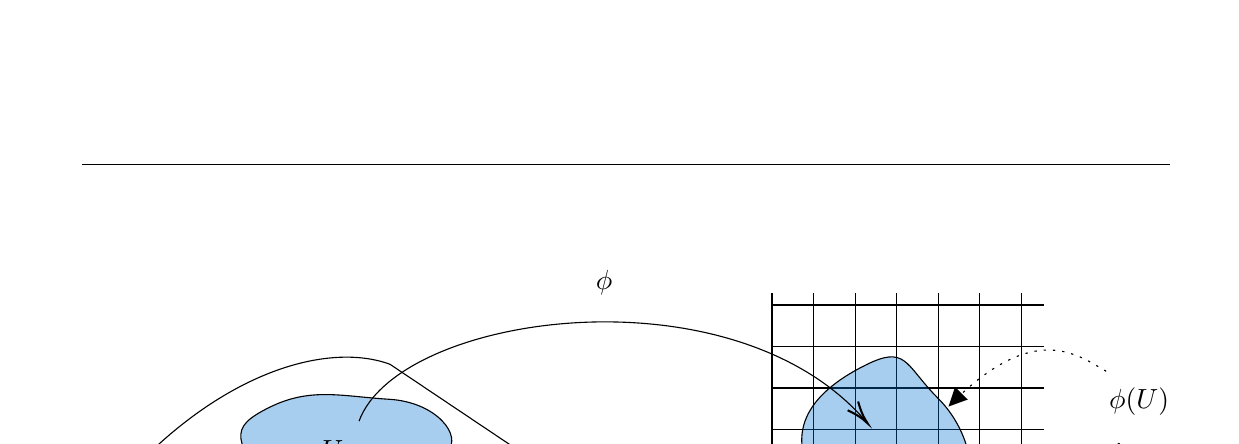
\begin{tikzpicture}[x=0.75pt,y=0.75pt,yscale=-1,xscale=1]
%uncomment if require: \path (0,300); %set diagram left start at 0, and has height of 300

%Curve Lines [id:da6045031736518898] 
\draw    (3.05,141.85) .. controls (54.14,81.78) and (108.24,68.22) .. (137.79,79.13) ;
%Straight Lines [id:da6673159815260592] 
\draw    (137.79,79.13) -- (236.5,145.28) ;
%Curve Lines [id:da7593498166846173] 
\draw    (101.76,208) .. controls (140.89,157.71) and (194.53,140.29) .. (236.5,145.28) ;
%Straight Lines [id:da5737020943480511] 
\draw    (3.05,141.85) -- (101.76,208) ;
%Shape: Polygon Curved [id:ds5933054421773951] 
\draw  [fill={rgb, 255:red, 2; green, 111; blue, 208 }  ,fill opacity=0.35 ] (79.5,100) .. controls (99.5,90) and (114.49,94.6) .. (137.5,96) .. controls (160.51,97.4) and (172.75,113.75) .. (165.5,121) .. controls (158.25,128.25) and (130.5,131) .. (130.5,148) .. controls (130.5,165) and (102.5,175) .. (82.5,145) .. controls (62.5,115) and (59.5,110) .. (79.5,100) -- cycle ;
%Shape: Grid [id:dp3824681513170989] 
\draw  [draw opacity=0] (321.88,170.55) -- (453,170.55) -- (453,44.55) -- (321.88,44.55) -- cycle ; \draw   (321.88,170.55) -- (321.88,44.55)(341.88,170.55) -- (341.88,44.55)(361.88,170.55) -- (361.88,44.55)(381.88,170.55) -- (381.88,44.55)(401.88,170.55) -- (401.88,44.55)(421.88,170.55) -- (421.88,44.55)(441.88,170.55) -- (441.88,44.55) ; \draw   (321.88,170.55) -- (453,170.55)(321.88,150.55) -- (453,150.55)(321.88,130.55) -- (453,130.55)(321.88,110.55) -- (453,110.55)(321.88,90.55) -- (453,90.55)(321.88,70.55) -- (453,70.55)(321.88,50.55) -- (453,50.55) ; \draw    ;
%Shape: Polygon Curved [id:ds5662007811356529] 
\draw  [fill={rgb, 255:red, 2; green, 111; blue, 208 }  ,fill opacity=0.35 ] (366.88,79.55) .. controls (386.15,69.92) and (385.93,78.85) .. (400.2,93.82) .. controls (400.74,94.39) and (401.3,94.97) .. (401.88,95.55) .. controls (417.88,111.55) and (421.13,135.31) .. (413.88,142.55) .. controls (406.63,149.8) and (397.88,126.55) .. (381.88,130.55) .. controls (365.88,134.55) and (363.88,167.55) .. (343.88,137.55) .. controls (323.88,107.55) and (346.88,89.55) .. (366.88,79.55) -- cycle ;
%Curve Lines [id:da8193544302387814] 
\draw    (122.88,106.55) .. controls (141.79,54.81) and (302.27,31.78) .. (366.92,106.42) ;
\draw [shift={(367.88,107.55)}, rotate = 229.9] [color={rgb, 255:red, 0; green, 0; blue, 0 }  ][line width=0.75]    (10.93,-3.29) .. controls (6.95,-1.4) and (3.31,-0.3) .. (0,0) .. controls (3.31,0.3) and (6.95,1.4) .. (10.93,3.29)   ;
%Curve Lines [id:da8020119262418375] 
\draw  [dash pattern={on 0.84pt off 2.51pt}]  (482.88,82.51) .. controls (469.09,74.63) and (448.51,58.02) .. (408.72,97.66) ;
\draw [shift={(406.88,99.51)}, rotate = 314.31] [fill={rgb, 255:red, 0; green, 0; blue, 0 }  ][line width=0.08]  [draw opacity=0] (8.93,-4.29) -- (0,0) -- (8.93,4.29) -- cycle    ;
%Curve Lines [id:da08576289583921382] 
\draw    (121.13,157.44) .. controls (171.32,177.68) and (284.02,182.88) .. (358.88,141.55) ;
\draw [shift={(118.88,156.51)}, rotate = 23.2] [color={rgb, 255:red, 0; green, 0; blue, 0 }  ][line width=0.75]    (10.93,-3.29) .. controls (6.95,-1.4) and (3.31,-0.3) .. (0,0) .. controls (3.31,0.3) and (6.95,1.4) .. (10.93,3.29)   ;

% Text Node
\draw (110,120.55) node    {$U$};
% Text Node
\draw (125,207.55) node    {$\mathcal{M}$};
% Text Node
\draw (331,186.55) node    {$\mathbb{R}^{n}$};
% Text Node
\draw (241,40) node    {$\phi $};
% Text Node
\draw (501,97) node    {$\phi ( U) \ $};
% Text Node
\draw (517,131) node   [align=left] {is an open\\subset of};
% Text Node
\draw (560,141.55) node    {$\mathbb{R}^{n}$};
% Text Node
\draw (248,186) node    {$\phi ^{-1}$};


\end{tikzpicture}

\caption{The definition of a Chart}
\label{fig:my_label 2}
\end{figure}


\begin{tcolorbox}
\textbf{Definition: Chart} \\ \\ 
Given a manifold $\mathcal{M}$ and a subset in it called $U$, we define a \textit{one-to-one} map $\phi$, called a \textit{chart}:

\begin{equation*}
    \phi: U \rightarrow \mathbb{R}^n
\end{equation*}

\textbf{Discussion:} \\
\begin{itemize}
    \item In general, since elements of $\mathbb{R}^n$ are just tuples of real numbers $(x^1,x^2,...,x^n)$, then $\phi(p)$ should just be tuples of real numbers $(\phi^1,\phi^2,...,\phi^n)$.
    \item  We can then write $\phi$ as a set of n functions, $\phi^{\mu}$ for $\mu \in \{1,...n\}$, which take points in $p$ and give real numbers. 
    \item This chart $\phi$ can be intuitively understood as \textit{a local coordinate system}. It assigns to each point $p$ within a subset $U$ of $\mathcal{M}$, a set of $n$ numbers.
    \item This assignment is unique within $U$, since $\phi$ is one-to-one. This makes sense since we want the set of numbers $\phi^{\mu}(p)$ to be representative of \textit{only} the point $p$.
    \item Sometimes we will say something like: \textit{consider a point $x^\mu$}. What we really mean, is that we have a chart called $x$, and in that chart the point $p$ we are considering gets mapped uniquely under $x$ to the point in $\mathbb{R}^n$ given by $x^{\mu}(p)$.
\end{itemize}

\end{tcolorbox}

A good example of a chart is how we use latitude and longitude to define positions on the surface of the earth, which is to a good approximation $\mathbb{S}^2$. We can call the chart $\phi$, and we find that it maps the surface to an open subset of $\mathbb{R}^2$ given by $(0,\pi)\cross(0,2\pi)$. We usually call $\phi^{0}(p)$ the latitude and $\phi^{1}(p)$ the longitude of point $p$.

\subsection{Chart transition maps}
Now that we've introduced charts, lets try and define a way in which two charts are consistent with each other. This will naturally lead us to conditions such that we can introduce a notion of \textit{smoothness} on the manifold. Let's say we've made two different charts, $\phi_1$ and $\phi_2$ on two different subsets $U_1$ and $U_2$ of the same manifold $\mathcal{M}$. Over the piece where the two subsets overlap, there must be a natural way to convert between coordinates given by the two different charts $\phi_1$ and $\phi_2$. 

\begin{figure}[h!]
\centering


\tikzset{every picture/.style={line width=0.75pt}} %set default line width to 0.75pt        

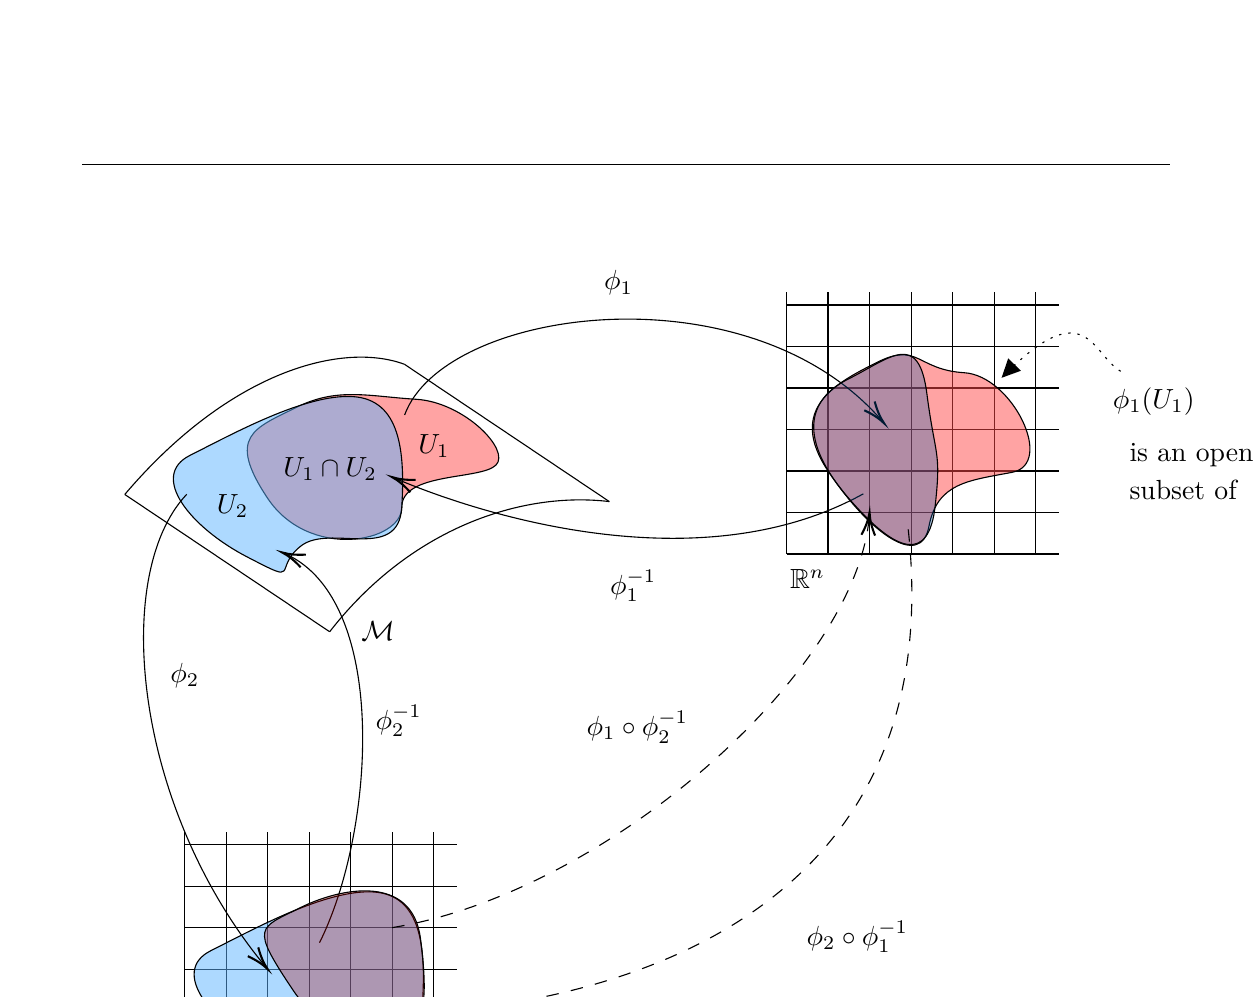
\begin{tikzpicture}[x=0.75pt,y=0.75pt,yscale=-1,xscale=1]
%uncomment if require: \path (0,475.69602966308594); %set diagram left start at 0, and has height of 475.69602966308594

%Curve Lines [id:da2896214219679667] 
\draw    (3.05,111.85) .. controls (54.14,51.78) and (108.24,38.22) .. (137.79,49.13) ;
%Straight Lines [id:da4179541205606838] 
\draw    (137.79,49.13) -- (236.5,115.28) ;
%Curve Lines [id:da9597228567215441] 
\draw    (101.76,178) .. controls (140.89,127.71) and (194.53,110.29) .. (236.5,115.28) ;
%Straight Lines [id:da04510421527961883] 
\draw    (3.05,111.85) -- (101.76,178) ;
%Shape: Polygon Curved [id:ds4775541445616551] 
\draw  [fill={rgb, 255:red, 255; green, 71; blue, 71 }  ,fill opacity=0.5 ] (85.5,70) .. controls (105.5,60) and (120.49,64.6) .. (143.5,66) .. controls (166.51,67.4) and (189.13,90.45) .. (181.88,97.7) .. controls (174.63,104.95) and (136.5,101) .. (136.5,118) .. controls (136.5,135) and (91.88,143.7) .. (71.88,113.7) .. controls (51.88,83.7) and (65.5,80) .. (85.5,70) -- cycle ;
%Shape: Grid [id:dp015367084248610885] 
\draw  [draw opacity=0] (321.88,140.55) -- (453,140.55) -- (453,14.55) -- (321.88,14.55) -- cycle ; \draw   (321.88,140.55) -- (321.88,14.55)(341.88,140.55) -- (341.88,14.55)(361.88,140.55) -- (361.88,14.55)(381.88,140.55) -- (381.88,14.55)(401.88,140.55) -- (401.88,14.55)(421.88,140.55) -- (421.88,14.55)(441.88,140.55) -- (441.88,14.55) ; \draw   (321.88,140.55) -- (453,140.55)(321.88,120.55) -- (453,120.55)(321.88,100.55) -- (453,100.55)(321.88,80.55) -- (453,80.55)(321.88,60.55) -- (453,60.55)(321.88,40.55) -- (453,40.55)(321.88,20.55) -- (453,20.55) ; \draw    ;
%Shape: Polygon Curved [id:ds9179792815682231] 
\draw  [fill={rgb, 255:red, 92; green, 179; blue, 255 }  ,fill opacity=0.5 ] (34.5,93) .. controls (54.5,83) and (89.87,63.3) .. (112.88,64.7) .. controls (135.89,66.1) and (138.12,91.3) .. (136.5,118) .. controls (134.88,144.7) and (101.88,125.7) .. (87.88,136.7) .. controls (73.88,147.7) and (88.88,155.88) .. (61.88,141.88) .. controls (34.88,127.88) and (14.5,103) .. (34.5,93) -- cycle ;
%Shape: Grid [id:dp44353478104543576] 
\draw  [draw opacity=0] (31.88,400.55) -- (163,400.55) -- (163,274.55) -- (31.88,274.55) -- cycle ; \draw   (31.88,400.55) -- (31.88,274.55)(51.88,400.55) -- (51.88,274.55)(71.88,400.55) -- (71.88,274.55)(91.88,400.55) -- (91.88,274.55)(111.88,400.55) -- (111.88,274.55)(131.88,400.55) -- (131.88,274.55)(151.88,400.55) -- (151.88,274.55) ; \draw   (31.88,400.55) -- (163,400.55)(31.88,380.55) -- (163,380.55)(31.88,360.55) -- (163,360.55)(31.88,340.55) -- (163,340.55)(31.88,320.55) -- (163,320.55)(31.88,300.55) -- (163,300.55)(31.88,280.55) -- (163,280.55) ; \draw    ;
%Shape: Polygon Curved [id:ds4406919657093047] 
\draw  [fill={rgb, 255:red, 255; green, 71; blue, 71 }  ,fill opacity=0.5 ] (365.5,48.2) .. controls (385.5,38.2) and (384.49,51.8) .. (407.5,53.2) .. controls (430.51,54.6) and (451.5,97.2) .. (430.5,101.2) .. controls (409.5,105.2) and (394.5,106.2) .. (390.5,127.2) .. controls (386.5,148.2) and (361.88,130.55) .. (341.88,100.55) .. controls (321.88,70.55) and (345.5,58.2) .. (365.5,48.2) -- cycle ;
%Shape: Polygon Curved [id:ds7424182116849432] 
\draw  [fill={rgb, 255:red, 92; green, 179; blue, 255 }  ,fill opacity=0.5 ] (44.5,331.67) .. controls (64.5,321.67) and (99.87,301.97) .. (122.88,303.37) .. controls (145.89,304.77) and (148.12,329.97) .. (146.5,356.67) .. controls (144.88,383.37) and (111.88,364.37) .. (97.88,375.37) .. controls (83.88,386.37) and (98.88,394.55) .. (71.88,380.55) .. controls (44.88,366.55) and (24.5,341.67) .. (44.5,331.67) -- cycle ;
%Curve Lines [id:da5281320057885546] 
\draw  [dash pattern={on 0.84pt off 2.51pt}]  (79.88,411.7) .. controls (88.66,394.15) and (113.23,409.1) .. (106.11,378.12) ;
\draw [shift={(105.5,375.65)}, rotate = 435.27] [fill={rgb, 255:red, 0; green, 0; blue, 0 }  ][line width=0.08]  [draw opacity=0] (8.93,-4.29) -- (0,0) -- (8.93,4.29) -- cycle    ;
%Curve Lines [id:da1691116666732393] 
\draw    (32.88,111.79) .. controls (-3.93,150.84) and (7.76,263.42) .. (70.93,339.41) ;
\draw [shift={(71.88,340.55)}, rotate = 229.9] [color={rgb, 255:red, 0; green, 0; blue, 0 }  ][line width=0.75]    (10.93,-3.29) .. controls (6.95,-1.4) and (3.31,-0.3) .. (0,0) .. controls (3.31,0.3) and (6.95,1.4) .. (10.93,3.29)   ;
%Curve Lines [id:da17388917049077435] 
\draw    (96.88,327.79) .. controls (123.61,274.33) and (130.74,163.05) .. (80.43,140.45) ;
\draw [shift={(78.88,139.79)}, rotate = 381.99] [color={rgb, 255:red, 0; green, 0; blue, 0 }  ][line width=0.75]    (10.93,-3.29) .. controls (6.95,-1.4) and (3.31,-0.3) .. (0,0) .. controls (3.31,0.3) and (6.95,1.4) .. (10.93,3.29)   ;
%Curve Lines [id:da35405636722682066] 
\draw    (137.88,73.55) .. controls (156.79,21.81) and (303.41,1.75) .. (367.92,76.42) ;
\draw [shift={(368.88,77.55)}, rotate = 229.9] [color={rgb, 255:red, 0; green, 0; blue, 0 }  ][line width=0.75]    (10.93,-3.29) .. controls (6.95,-1.4) and (3.31,-0.3) .. (0,0) .. controls (3.31,0.3) and (6.95,1.4) .. (10.93,3.29)   ;
%Curve Lines [id:da9415974477100371] 
\draw  [dash pattern={on 0.84pt off 2.51pt}]  (482.88,52.51) .. controls (469.09,44.63) and (466.57,14.57) .. (427.32,53.8) ;
\draw [shift={(425.5,55.65)}, rotate = 314.31] [fill={rgb, 255:red, 0; green, 0; blue, 0 }  ][line width=0.08]  [draw opacity=0] (8.93,-4.29) -- (0,0) -- (8.93,4.29) -- cycle    ;
%Curve Lines [id:da8468782246975544] 
\draw    (134.12,104.46) .. controls (183.94,125.36) and (284.02,152.88) .. (358.88,111.55) ;
\draw [shift={(131.88,103.51)}, rotate = 23.2] [color={rgb, 255:red, 0; green, 0; blue, 0 }  ][line width=0.75]    (10.93,-3.29) .. controls (6.95,-1.4) and (3.31,-0.3) .. (0,0) .. controls (3.31,0.3) and (6.95,1.4) .. (10.93,3.29)   ;
%Shape: Polygon Curved [id:ds7843896932131351] 
\draw  [fill={rgb, 255:red, 172; green, 0; blue, 0 }  ,fill opacity=0.3 ] (87.5,311) .. controls (107.5,301) and (141.5,294.76) .. (145.5,325.76) .. controls (149.5,356.76) and (147.5,370.76) .. (133.5,370.76) .. controls (119.5,370.76) and (103.5,379.76) .. (83.5,349.76) .. controls (63.5,319.76) and (67.5,321) .. (87.5,311) -- cycle ;
%Shape: Polygon Curved [id:ds19585008898624823] 
\draw  [fill={rgb, 255:red, 0; green, 88; blue, 172 }  ,fill opacity=0.3 ] (351.5,56.31) .. controls (371.5,46.31) and (385.5,32.31) .. (389.5,63.31) .. controls (393.5,94.31) and (396.5,90.31) .. (393.5,117.31) .. controls (390.5,144.31) and (375.5,141.31) .. (351.5,113.31) .. controls (327.5,85.31) and (331.5,66.31) .. (351.5,56.31) -- cycle ;
%Curve Lines [id:da6766796381178022] 
\draw  [dash pattern={on 4.5pt off 4.5pt}]  (380.5,128.65) .. controls (403.27,336.55) and (197.68,359.21) .. (145.05,361.58) ;
\draw [shift={(143.5,361.65)}, rotate = 357.71000000000004] [color={rgb, 255:red, 0; green, 0; blue, 0 }  ][line width=0.75]    (10.93,-3.29) .. controls (6.95,-1.4) and (3.31,-0.3) .. (0,0) .. controls (3.31,0.3) and (6.95,1.4) .. (10.93,3.29)   ;
%Curve Lines [id:da36354948965215694] 
\draw  [dash pattern={on 4.5pt off 4.5pt}]  (131.88,320.55) .. controls (235.36,303.64) and (356.28,196.72) .. (361.81,121.68) ;
\draw [shift={(361.88,120.55)}, rotate = 453.34] [color={rgb, 255:red, 0; green, 0; blue, 0 }  ][line width=0.75]    (10.93,-3.29) .. controls (6.95,-1.4) and (3.31,-0.3) .. (0,0) .. controls (3.31,0.3) and (6.95,1.4) .. (10.93,3.29)   ;

% Text Node
\draw (152,88.55) node    {$U_{1}$};
% Text Node
\draw (125,177.55) node    {$\mathcal{M}$};
% Text Node
\draw (332,152.55) node    {$\mathbb{R}^{n}$};
% Text Node
\draw (241,10) node    {$\phi _{1}$};
% Text Node
\draw (501,67) node    {$\phi _{1}( U_{1}) \ $};
% Text Node
\draw (517,101) node   [align=left] {is an open\\subset of};
% Text Node
\draw (560,111.55) node    {$\mathbb{R}^{n}$};
% Text Node
\draw (248,156) node    {$\phi ^{-1}_{1}$};
% Text Node
\draw (55,117.55) node    {$U_{2}$};
% Text Node
\draw (102,99.55) node    {$U_{1} \cap U_{2}$};
% Text Node
\draw (41,416.55) node    {$\mathbb{R}^{n}$};
% Text Node
\draw (80,424) node    {$\phi _{2}( U_{2}) \ $};
% Text Node
\draw (143,435) node   [align=left] {is an open\\subset of};
% Text Node
\draw (186,443.55) node    {$\mathbb{R}^{n}$};
% Text Node
\draw (32,199) node    {$\phi _{2}$};
% Text Node
\draw (135,221) node    {$\phi ^{-1}_{2}$};
% Text Node
\draw (356,325) node    {$\phi _{2} \circ \phi ^{-1}_{1}$};
% Text Node
\draw (250,224) node    {$\phi _{1} \circ \phi ^{-1}_{2}$};


\end{tikzpicture}

\caption{Chart Transition Maps $\phi_1\circ\phi_2^{-1}$ and $\phi_2\circ\phi_1^{-1}$}
\label{fig:my_label 3}
\end{figure}

\begin{tcolorbox}
\textbf{Definition: Chart Transition Maps} \\ \\ 
Given a manifold $\mathcal{M}$, two charts $(\phi_1,U_1)$ and $(\phi_2,U_2)$ such that $U_1$ and $U_2$ overlap, we can identify the coordinates assigned to the same point by the two different functions using something called a \textit{chart transition map} between chart 1 and chart 2 defined as:

\begin{align*}
    \phi_{1\rightarrow 2} &= \phi_2\circ\phi_1^{-1} : \mathbb{R}^n \rightarrow \mathbb{R}^n \\
    \phi_{2\rightarrow 1} &= \phi_1\circ\phi_2^{-1} : \mathbb{R}^n \rightarrow \mathbb{R}^n
\end{align*}

\end{tcolorbox}

The natural way to construct a map from the chart functions $\phi_1^{\mu}$ to $\phi_2^{\nu}$ must be by inverting $\phi_1$, so that it takes a coordinate in $\mathbb{R}^n$ and gives a point on the manifold, $p$. Once we have that point, we can use the $\phi_2$ map to get the coordinates $\phi_2^{\mu}(p)$. So given a point $\phi^{\mu}(p) = (\phi^{1}_1(p),\phi^{2}_1(p),...,\phi^{n}_1(p))$ in a subset of $\mathbb{R}^n$ related to a chart $\phi_1$, we can get the coordinates of the point in the manifold $p$ using the inverse map $\phi_{1\rightarrow 2} = \phi_2\circ\phi_1^{-1}$. These chart transition functions are also known as \textit{coordinate transformations}.

An obvious fact here is, that to be able to completely describe a manifold, we need to have every point in the manifold covered by at least one chart. So to characterise a manifold, a really important object one needs is a collection of charts $(\phi_{\alpha},U_{\alpha})$ such that $\bigcup_{\alpha} U_{\alpha} = \mathcal{M}$. Such a collection is appropriately referred to as an \textit{atlas} \\

\begin{tcolorbox}
\textbf{Definition: Atlas} \\ \\ 
Given a manifold $\mathcal{M}$, an atlas $\mathcal{A}$ is defined as a collection of charts and all possible chart transition maps between those charts

\begin{align*}
    \mathcal{A} = (\{(\phi_{\alpha}, U_{\alpha}) ;\, \forall\, \alpha\} , \{(\phi_{\beta}\circ\phi_{\alpha}^{-1}, U_{\alpha}\cup U_{\beta}) ;\, \forall\, \alpha\ , \beta\} )
\end{align*}

such that the subsets $U_{\alpha}$ completely cover $\mathcal{M}$. I.e.:

\begin{align*}
    \bigcup_{\alpha} U_{\alpha} \cong \mathcal{M}
\end{align*}

There is also the \textbf{Maximal Atlas}, which is defined to be the largest consistent union of all atlases. 

\end{tcolorbox}

\subsection{Smooth Atlases}
Now what we want to do is get a definition of differentiability on a manifold. We know how to do that in $\mathbb{R}^n$ using all the epsilon-delta machinery from real analysis, but it's not too straightforward in the case of a manifold. 

A naive first attempt at this would be the following case: 
Define a manifold $\mathcal{M}$ and a coordinate chart $(\phi,U)$. We can assign sets of numbers to points in $U$. If we represent $U$ as a region in $\mathbb{R}^n$, and pick a differentiable function within $U$ on $\mathbb{R}^n$ \sn{we can say whats differentiable there since we have a notion of differentiability in $\mathbb{R}^n$} (we know what differentiability means in $\mathbb{R}^n$), we can \textit{assert} that this function is differentiable. 

However it isn't that simple, because let's say we asserted the differentiability of the function on a chart $(\phi_1,U_1)$, and when we transformed to a different chart $(\phi_2,U_2)$ using the chart transition function $\phi_2\circ\phi_1^{-1}$ we find that the new function on a subset of $\mathbb{R}^n$ is not differentiable anymore. We had a differentiable function on a piece of $\mathbb{R}^n$ that got mapped to a non-differentiable function on some other piece of $\mathbb{R}^n$ using the map  $\phi_2\circ\phi_1^{-1}$. This could only mean that the function $\phi_2\circ\phi_1^{-1}$ was \textbf{not} a differentiable function. 

So the simple way to be able to say anything about the differentiability of things on manifolds is to define them in a way that differentiability is preserved between charts. Hence, this could  only be if we took our atlas $\mathcal{A}$ and threw away all the non-differentiable chart transition functions such that in the new atlas $\mathcal{A}_{differentiable}$,  all the remaining chart transition functions are \textit{differentiable}.

We could go even further, and say that we only keep those chart transition functions that are \textit{smooth}, or infinitely differentiable . This means if we write an infinitely differentiable function in some patch on a given chart, when we transform our chart, it remains infinitely differentiable. If we have a twice-differentiable function $f \in \mathcal{C}^2$ in some chart, then it shall be twice differentiable in all charts. This gives us a \textit{coordinate invariant} notion of continuity/differentiability/smoothness of a function. \sn{If we would like a more restrictive setup we could make all of our transition maps only continuous ($\mathcal{C}^{0}$) as opposed to smooth $\mathcal{C}^{\infty}$, which would be a different type of manifold that has a defined notion of continuity but a version of differentiability that is not coordinate invariant.} Which brings us to the definition of a smooth atlas:\\

\begin{tcolorbox}
\textbf{Definition: Smooth Atlas} \\ \\ 
Given a manifold $\mathcal{M}$, a smooth atlas $\mathcal{A}$ is defined as an atlas such that all chart transition maps between its charts are \textbf{smooth}, or infinitely differentiable.
\end{tcolorbox}

We can now state the definition of a smooth manifold. A smooth $n$-dimensional manifold is a space of points $\mathcal{M}$ equipped with a smooth atlas $\mathcal{A}$ such that the charts in it map to $\mathbb{R}^n$. A more fleshed out version of the definition of a manifold is given below:
\\
\begin{tcolorbox}
\textbf{Definition: A Smooth $n$-dimensional Manifold} \\

A Smooth $n$-dimensional Manifold $\mathcal{M}$ is 
\begin{enumerate}
    \item A space of points : $\mathcal{M}$ (with a topology)
    \item a collection of open subsets $U_{\alpha}$ of $\mathcal{M}$ that cover $\mathcal{M}$. i.e. $\bigcup_{\alpha} U_{\alpha} \cong \mathcal{M}$
    \item charts: ($\phi_{\alpha}:U_{\alpha} \rightarrow \mathbb{R}^n$)
    \item \textit{smooth} chart transition maps: $\phi_{\alpha\rightarrow \beta} = \phi_{\beta}\circ\phi_{\alpha}^{-1} \in \mathcal{C}^{\infty}$
    \item The largest possible consistent collection of items 2-4, called a smooth maximal atlas $\mathcal{A}$
\end{enumerate}

\end{tcolorbox}
%\vspace{\fill}
%\pagebreak

\section{Examples of Atlases on $\mathbb{S}^2$}
We can now look at some examples of constructing atlases on $\mathbb{S}$. Here are some visual representations, shown in \textbf{Figure 9} and \textbf{Figure 10} on how we construct the atlas. In both cases we choose two open sets $U_{north}$ and $U_{south}$, and construct maps from these to some subsets of $\mathbb{R}^n$. The chart transition maps should then

\begin{figure}[h!]
\centering


\tikzset{every picture/.style={line width=0.75pt}} %set default line width to 0.75pt        

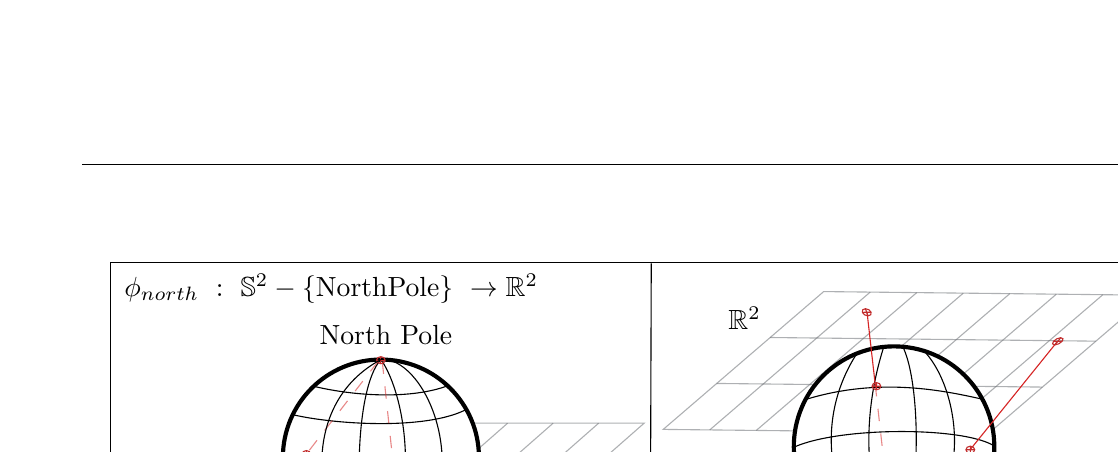
\begin{tikzpicture}[x=0.75pt,y=0.75pt,yscale=-0.8,xscale=0.8]
%uncomment if require: \path (0,300); %set diagram left start at 0, and has height of 300

%Shape: Grid [id:dp6743053147024749] 
\draw  [draw opacity=0] (447.63,40.76) -- (643.8,42.95) -- (547.16,125.95) -- (351,123.76) -- cycle ; \draw  [color={rgb, 255:red, 102; green, 106; blue, 111 }  ,draw opacity=0.53 ] (475.66,41.07) -- (379.02,124.07)(503.68,41.38) -- (407.04,124.39)(531.71,41.7) -- (435.07,124.7)(559.73,42.01) -- (463.09,125.01)(587.75,42.32) -- (491.12,125.32)(615.78,42.63) -- (519.14,125.64) ; \draw  [color={rgb, 255:red, 102; green, 106; blue, 111 }  ,draw opacity=0.53 ] (415.42,68.42) -- (611.59,70.62)(383.21,96.09) -- (579.38,98.28) ; \draw  [color={rgb, 255:red, 102; green, 106; blue, 111 }  ,draw opacity=0.53 ] (447.63,40.76) -- (643.8,42.95) -- (547.16,125.95) -- (351,123.76) -- cycle ;
%Shape: Ellipse [id:dp9425545016257557] 
\draw  [fill={rgb, 255:red, 255; green, 255; blue, 255 }  ,fill opacity=1 ][line width=1.5]  (550.39,133.77) .. controls (550.58,167.11) and (523.71,194.3) .. (490.37,194.5) .. controls (457.03,194.7) and (429.84,167.83) .. (429.64,134.49) .. controls (429.44,101.14) and (456.31,73.95) .. (489.65,73.76) .. controls (523,73.56) and (550.19,100.43) .. (550.39,133.77) -- cycle ;
%Curve Lines [id:da3664132357105905] 
\draw    (490.37,194.5) .. controls (465.19,197.04) and (432.01,132.42) .. (468.06,77.34) ;
%Curve Lines [id:da2063339465896168] 
\draw    (490.37,194.5) .. controls (480,180.43) and (464.81,132.82) .. (484.13,73.07) ;
%Curve Lines [id:da03600208468621302] 
\draw    (490.37,194.5) .. controls (506.81,176.81) and (506.93,95.72) .. (494.87,73.13) ;
%Curve Lines [id:da3917673051762569] 
\draw    (550.39,133.77) .. controls (532.13,122.1) and (457.59,121.95) .. (429.64,134.49) ;
%Curve Lines [id:da21622650053014336] 
\draw    (544.28,160.19) .. controls (518.61,154.38) and (463.13,151.13) .. (438.16,163.8) ;
%Curve Lines [id:da806841089210655] 
\draw    (542.17,105.35) .. controls (516.49,99.54) and (478.88,92.6) .. (436.03,105.98) ;
%Curve Lines [id:da9208356227830126] 
\draw    (530.67,177.57) .. controls (504.99,171.76) and (471.59,170.17) .. (448.98,178.65) ;
%Straight Lines [id:da9448878564052738] 
\draw [color={rgb, 255:red, 213; green, 36; blue, 36 }  ,draw opacity=1 ]   (535.62,136.25) -- (588.3,70.94) ;
%Straight Lines [id:da5058477647271051] 
\draw [color={rgb, 255:red, 213; green, 36; blue, 36 }  ,draw opacity=0.54 ] [dash pattern={on 4.5pt off 4.5pt}]  (492.15,193.3) -- (535.94,136.02) ;
%Flowchart: Or [id:dp2531197296181813] 
\draw  [color={rgb, 255:red, 194; green, 45; blue, 45 }  ,draw opacity=1 ] (492.99,194.12) .. controls (493,195.31) and (491.83,196.28) .. (490.38,196.29) .. controls (488.93,196.3) and (487.75,195.34) .. (487.75,194.15) .. controls (487.74,192.96) and (488.91,191.98) .. (490.36,191.97) .. controls (491.8,191.96) and (492.98,192.92) .. (492.99,194.12) -- cycle ; \draw  [color={rgb, 255:red, 194; green, 45; blue, 45 }  ,draw opacity=1 ] (492.99,194.12) -- (487.75,194.15) ; \draw  [color={rgb, 255:red, 194; green, 45; blue, 45 }  ,draw opacity=1 ] (490.38,196.29) -- (490.36,191.97) ;
%Flowchart: Or [id:dp23482727896505917] 
\draw  [color={rgb, 255:red, 194; green, 45; blue, 45 }  ,draw opacity=1 ] (538.56,136) .. controls (538.57,137.2) and (537.4,138.17) .. (535.95,138.18) .. controls (534.5,138.19) and (533.32,137.23) .. (533.32,136.04) .. controls (533.31,134.84) and (534.48,133.87) .. (535.93,133.86) .. controls (537.37,133.85) and (538.55,134.81) .. (538.56,136) -- cycle ; \draw  [color={rgb, 255:red, 194; green, 45; blue, 45 }  ,draw opacity=1 ] (538.56,136) -- (533.32,136.04) ; \draw  [color={rgb, 255:red, 194; green, 45; blue, 45 }  ,draw opacity=1 ] (535.95,138.18) -- (535.93,133.86) ;
%Flowchart: Or [id:dp27406611804482517] 
\draw  [color={rgb, 255:red, 194; green, 45; blue, 45 }  ,draw opacity=1 ] (591.24,70.7) .. controls (590.24,71.89) and (588.26,72.87) .. (586.81,72.88) .. controls (585.36,72.89) and (585,71.92) .. (586,70.73) .. controls (587,69.53) and (588.99,68.55) .. (590.43,68.54) .. controls (591.88,68.53) and (592.24,69.5) .. (591.24,70.7) -- cycle ; \draw  [color={rgb, 255:red, 194; green, 45; blue, 45 }  ,draw opacity=1 ] (591.24,70.7) -- (586,70.73) ; \draw  [color={rgb, 255:red, 194; green, 45; blue, 45 }  ,draw opacity=1 ] (586.81,72.88) -- (590.43,68.54) ;
%Curve Lines [id:da27814450720477857] 
\draw    (490.37,194.5) .. controls (540.74,166.95) and (529.62,100.83) .. (509.21,77.81) ;
%Straight Lines [id:da18733784273598086] 
\draw [color={rgb, 255:red, 213; green, 36; blue, 36 }  ,draw opacity=1 ]   (478.84,98.24) -- (473.75,53.24) ;
%Straight Lines [id:da8446436111405344] 
\draw [color={rgb, 255:red, 213; green, 36; blue, 36 }  ,draw opacity=0.54 ] [dash pattern={on 4.5pt off 4.5pt}]  (489.53,193.32) -- (478.84,98.24) ;
%Flowchart: Or [id:dp19975421061942722] 
\draw  [color={rgb, 255:red, 194; green, 45; blue, 45 }  ,draw opacity=1 ] (476.16,53.22) .. controls (476.6,54.41) and (475.78,55.38) .. (474.33,55.39) .. controls (472.88,55.4) and (471.36,54.44) .. (470.92,53.25) .. controls (470.49,52.06) and (471.31,51.09) .. (472.76,51.08) .. controls (474.2,51.07) and (475.73,52.03) .. (476.16,53.22) -- cycle ; \draw  [color={rgb, 255:red, 194; green, 45; blue, 45 }  ,draw opacity=1 ] (476.16,53.22) -- (470.92,53.25) ; \draw  [color={rgb, 255:red, 194; green, 45; blue, 45 }  ,draw opacity=1 ] (474.33,55.39) -- (472.76,51.08) ;
%Flowchart: Or [id:dp4818686918630233] 
\draw  [color={rgb, 255:red, 194; green, 45; blue, 45 }  ,draw opacity=1 ] (482.04,97.74) .. controls (482.04,98.93) and (480.88,99.9) .. (479.43,99.91) .. controls (477.98,99.92) and (476.8,98.96) .. (476.79,97.77) .. controls (476.79,96.58) and (477.95,95.6) .. (479.4,95.59) .. controls (480.85,95.58) and (482.03,96.54) .. (482.04,97.74) -- cycle ; \draw  [color={rgb, 255:red, 194; green, 45; blue, 45 }  ,draw opacity=1 ] (482.04,97.74) -- (476.79,97.77) ; \draw  [color={rgb, 255:red, 194; green, 45; blue, 45 }  ,draw opacity=1 ] (479.43,99.91) -- (479.4,95.59) ;
%Shape: Grid [id:dp0029032340778514243] 
\draw  [draw opacity=0] (147.67,120.01) -- (339.51,120.01) -- (214.73,229.64) -- (22.88,229.64) -- cycle ; \draw  [color={rgb, 255:red, 102; green, 106; blue, 111 }  ,draw opacity=0.53 ] (175.07,120.01) -- (50.29,229.64)(202.48,120.01) -- (77.69,229.64)(229.89,120.01) -- (105.1,229.64)(257.29,120.01) -- (132.51,229.64)(284.7,120.01) -- (159.91,229.64)(312.11,120.01) -- (187.32,229.64) ; \draw  [color={rgb, 255:red, 102; green, 106; blue, 111 }  ,draw opacity=0.53 ] (116.47,147.42) -- (308.32,147.42)(85.27,174.83) -- (277.12,174.83)(54.08,202.23) -- (245.92,202.23) ; \draw  [color={rgb, 255:red, 102; green, 106; blue, 111 }  ,draw opacity=0.53 ] (147.67,120.01) -- (339.51,120.01) -- (214.73,229.64) -- (22.88,229.64) -- cycle ;
%Shape: Ellipse [id:dp7792534377323779] 
\draw  [fill={rgb, 255:red, 255; green, 255; blue, 255 }  ,fill opacity=1 ][line width=1.5]  (121.94,140.74) .. controls (121.94,108.14) and (148.37,81.7) .. (180.98,81.7) .. controls (213.58,81.7) and (240.02,108.14) .. (240.02,140.74) .. controls (240.02,173.35) and (213.58,199.79) .. (180.98,199.79) .. controls (148.37,199.79) and (121.94,173.35) .. (121.94,140.74) -- cycle ;
%Curve Lines [id:da12914477605341568] 
\draw    (180.98,81.7) .. controls (205.61,79.37) and (237.68,142.76) .. (202.11,196.4) ;
%Curve Lines [id:da1834224204179713] 
\draw    (180.98,81.7) .. controls (191.03,95.52) and (205.61,142.17) .. (186.37,200.48) ;
%Curve Lines [id:da4965782691226883] 
\draw    (180.98,81.7) .. controls (164.79,98.91) and (164.21,178.21) .. (175.87,200.37) ;
%Curve Lines [id:da29854012910446404] 
\draw    (121.94,140.74) .. controls (139.72,152.26) and (212.61,152.84) .. (240.02,140.74) ;
%Curve Lines [id:da9126386469294427] 
\draw    (128.06,114.94) .. controls (153.13,120.77) and (207.36,124.27) .. (231.85,112.03) ;
%Curve Lines [id:da12541240725268454] 
\draw    (129.81,168.59) .. controls (154.88,174.42) and (191.62,181.42) .. (233.6,168.59) ;
%Curve Lines [id:da6232105894950362] 
\draw    (141.47,98.03) .. controls (166.54,103.86) and (199.2,105.61) .. (221.36,97.45) ;
%Straight Lines [id:da39705727724579254] 
\draw [color={rgb, 255:red, 213; green, 36; blue, 36 }  ,draw opacity=1 ]   (136.39,138.41) -- (84.49,201.97) ;
%Straight Lines [id:da05954217401708184] 
\draw [color={rgb, 255:red, 213; green, 36; blue, 36 }  ,draw opacity=0.54 ] [dash pattern={on 4.5pt off 4.5pt}]  (179.23,82.87) -- (136.08,138.63) ;
%Flowchart: Or [id:dp5823724267788954] 
\draw  [color={rgb, 255:red, 194; green, 45; blue, 45 }  ,draw opacity=1 ] (178.41,82.07) .. controls (178.41,80.9) and (179.56,79.95) .. (180.98,79.95) .. controls (182.39,79.95) and (183.54,80.9) .. (183.54,82.07) .. controls (183.54,83.23) and (182.39,84.18) .. (180.98,84.18) .. controls (179.56,84.18) and (178.41,83.23) .. (178.41,82.07) -- cycle ; \draw  [color={rgb, 255:red, 194; green, 45; blue, 45 }  ,draw opacity=1 ] (178.41,82.07) -- (183.54,82.07) ; \draw  [color={rgb, 255:red, 194; green, 45; blue, 45 }  ,draw opacity=1 ] (180.98,79.95) -- (180.98,84.18) ;
%Flowchart: Or [id:dp6981483886810014] 
\draw  [color={rgb, 255:red, 194; green, 45; blue, 45 }  ,draw opacity=1 ] (133.51,138.63) .. controls (133.51,137.46) and (134.66,136.52) .. (136.08,136.52) .. controls (137.49,136.52) and (138.64,137.46) .. (138.64,138.63) .. controls (138.64,139.79) and (137.49,140.74) .. (136.08,140.74) .. controls (134.66,140.74) and (133.51,139.79) .. (133.51,138.63) -- cycle ; \draw  [color={rgb, 255:red, 194; green, 45; blue, 45 }  ,draw opacity=1 ] (133.51,138.63) -- (138.64,138.63) ; \draw  [color={rgb, 255:red, 194; green, 45; blue, 45 }  ,draw opacity=1 ] (136.08,136.52) -- (136.08,140.74) ;
%Flowchart: Or [id:dp8084920539236542] 
\draw  [color={rgb, 255:red, 194; green, 45; blue, 45 }  ,draw opacity=1 ] (81.61,202.19) .. controls (82.6,201.02) and (84.55,200.08) .. (85.96,200.08) .. controls (87.38,200.08) and (87.73,201.02) .. (86.74,202.19) .. controls (85.76,203.35) and (83.81,204.3) .. (82.39,204.3) .. controls (80.98,204.3) and (80.63,203.35) .. (81.61,202.19) -- cycle ; \draw  [color={rgb, 255:red, 194; green, 45; blue, 45 }  ,draw opacity=1 ] (81.61,202.19) -- (86.74,202.19) ; \draw  [color={rgb, 255:red, 194; green, 45; blue, 45 }  ,draw opacity=1 ] (85.96,200.08) -- (82.39,204.3) ;
%Curve Lines [id:da006877447169351569] 
\draw    (180.98,81.7) .. controls (131.56,108.35) and (142.05,173.08) .. (161.88,195.7) ;
%Straight Lines [id:da12962070826458394] 
\draw [color={rgb, 255:red, 213; green, 36; blue, 36 }  ,draw opacity=1 ]   (191.69,175.9) -- (196.41,219.94) ;
%Straight Lines [id:da371253644803736] 
\draw [color={rgb, 255:red, 213; green, 36; blue, 36 }  ,draw opacity=0.54 ] [dash pattern={on 4.5pt off 4.5pt}]  (181.79,82.87) -- (191.69,175.9) ;
%Flowchart: Or [id:dp6958552356937173] 
\draw  [color={rgb, 255:red, 194; green, 45; blue, 45 }  ,draw opacity=1 ] (194.05,219.94) .. controls (193.63,218.78) and (194.44,217.83) .. (195.85,217.83) .. controls (197.27,217.83) and (198.76,218.78) .. (199.18,219.94) .. controls (199.59,221.11) and (198.78,222.05) .. (197.37,222.05) .. controls (195.95,222.05) and (194.47,221.11) .. (194.05,219.94) -- cycle ; \draw  [color={rgb, 255:red, 194; green, 45; blue, 45 }  ,draw opacity=1 ] (194.05,219.94) -- (199.18,219.94) ; \draw  [color={rgb, 255:red, 194; green, 45; blue, 45 }  ,draw opacity=1 ] (195.85,217.83) -- (197.37,222.05) ;
%Flowchart: Or [id:dp7542563882878988] 
\draw  [color={rgb, 255:red, 194; green, 45; blue, 45 }  ,draw opacity=1 ] (188.56,176.38) .. controls (188.56,175.21) and (189.71,174.27) .. (191.13,174.27) .. controls (192.54,174.27) and (193.69,175.21) .. (193.69,176.38) .. controls (193.69,177.54) and (192.54,178.49) .. (191.13,178.49) .. controls (189.71,178.49) and (188.56,177.54) .. (188.56,176.38) -- cycle ; \draw  [color={rgb, 255:red, 194; green, 45; blue, 45 }  ,draw opacity=1 ] (188.56,176.38) -- (193.69,176.38) ; \draw  [color={rgb, 255:red, 194; green, 45; blue, 45 }  ,draw opacity=1 ] (191.13,174.27) -- (191.13,178.49) ;
%Straight Lines [id:da6239272721454003] 
\draw    (343.79,23.72) -- (343.03,259.72) ;
%Shape: Rectangle [id:dp43166433284321837] 
\draw   (18,23) -- (656.79,23) -- (656.79,260.72) -- (18,260.72) -- cycle ;

% Text Node
\draw (489.79,209.37) node  [rotate=-359.2] [align=left] {South Pole};
% Text Node
\draw (183.99,67.18) node   [align=left] {North Pole};
% Text Node
\draw (245,229) node    {$\mathbb{R}^{2}$};
% Text Node
\draw (400,57) node    {$\mathbb{R}^{2}$};
% Text Node
\draw (151,39) node    {$\phi _{north} \ :\ \mathbb{S}^{2} -\{\text{NorthPole}\} \ \rightarrow \mathbb{R}^{2}$};
% Text Node
\draw (498,241) node    {$\phi _{south} \ :\ \mathbb{S}^{2} -\{\text{SouthPole}\} \ \rightarrow \mathbb{R}^{2}$};


\end{tikzpicture}

\caption{Stereographic Projections: The first is $\phi_{north}$ which maps all points \textbf{but} the north pole to a point in $\mathbb{R}^2$. The second is $\phi_{south}$ which maps all points \textbf{but} the south pole to a point in $\mathbb{R}^2$.}

\end{figure}
\begin{figure}[h!]
\centering


\tikzset{every picture/.style={line width=0.75pt}} %set default line width to 0.75pt        

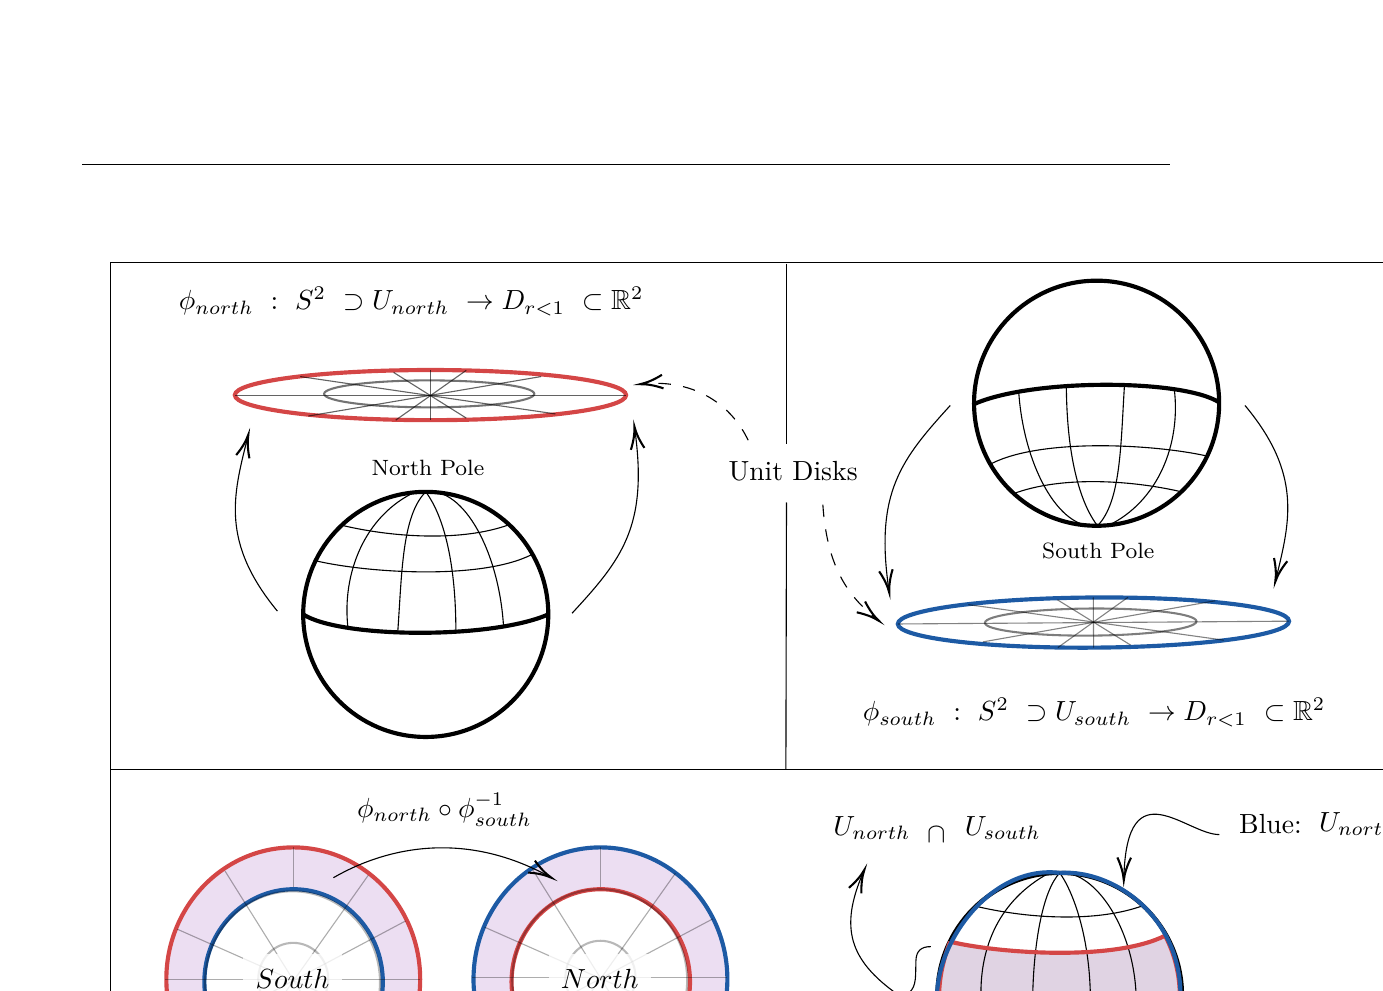
\begin{tikzpicture}[x=0.75pt,y=0.75pt,yscale=-1,xscale=1]
%uncomment if require: \path (0,491.9375); %set diagram left start at 0, and has height of 491.9375

%Shape: Polygon Curved [id:ds023966166008199785] 
\draw  [draw opacity=0][fill={rgb, 255:red, 102; green, 36; blue, 114 }  ,fill opacity=0.2 ] (422.61,350.46) .. controls (422.92,345.72) and (429.83,358.23) .. (480.83,356.23) .. controls (531.83,354.23) and (522.96,343.89) .. (526.2,347.55) .. controls (529.43,351.2) and (537.83,389.23) .. (531.5,394.45) .. controls (525.17,399.66) and (503.56,401.45) .. (478.83,402.23) .. controls (454.11,403.01) and (428.64,400.14) .. (422.36,397) .. controls (416.07,393.86) and (415.62,382.13) .. (416.83,370.23) .. controls (418.05,358.33) and (422.3,355.2) .. (422.61,350.46) -- cycle ;
%Shape: Ellipse [id:dp2648686510145266] 
\draw  [fill={rgb, 255:red, 255; green, 255; blue, 255 }  ,fill opacity=1 ][line width=1.5]  (110.94,192.74) .. controls (110.94,160.14) and (137.37,133.7) .. (169.98,133.7) .. controls (202.58,133.7) and (229.02,160.14) .. (229.02,192.74) .. controls (229.02,225.35) and (202.58,251.79) .. (169.98,251.79) .. controls (137.37,251.79) and (110.94,225.35) .. (110.94,192.74) -- cycle ;
%Curve Lines [id:da9237854012998243] 
\draw [line width=1.5]    (110.94,192.74) .. controls (128.72,204.26) and (201.61,204.84) .. (229.02,192.74) ;
%Curve Lines [id:da04122612033365991] 
\draw    (117.06,166.94) .. controls (142.13,172.77) and (196.36,176.27) .. (220.85,164.03) ;
%Curve Lines [id:da869429699713544] 
\draw    (130.47,150.03) .. controls (155.54,155.86) and (188.2,157.61) .. (210.36,149.45) ;
%Straight Lines [id:da5498697318616299] 
\draw    (343.79,23.72) -- (343.79,110.83) ;
%Shape: Rectangle [id:dp545596124429909] 
\draw   (18,23) -- (656.79,23) -- (656.79,267.27) -- (18,267.27) -- cycle ;
%Curve Lines [id:da039387430220944264] 
\draw    (164.98,133.7) .. controls (140.5,145.16) and (129.5,173.16) .. (132.5,199.16) ;
%Curve Lines [id:da7934563134568218] 
\draw    (169.98,133.7) .. controls (158.5,145.16) and (158.5,173.16) .. (156.5,201.16) ;
%Curve Lines [id:da36889608769204973] 
\draw    (169.98,133.7) .. controls (172.5,137.16) and (184.5,153.16) .. (184.5,201.16) ;
%Curve Lines [id:da14192555636374338] 
\draw    (169.98,133.7) .. controls (188.5,131.16) and (205.5,163.16) .. (207.5,199.16) ;
%Shape: Ellipse [id:dp5496551580252034] 
\draw  [color={rgb, 255:red, 212; green, 70; blue, 70 }  ,draw opacity=1 ][line width=1.5]  (78,87.08) .. controls (78,80.41) and (120.2,75) .. (172.25,75) .. controls (224.3,75) and (266.5,80.41) .. (266.5,87.08) .. controls (266.5,93.75) and (224.3,99.16) .. (172.25,99.16) .. controls (120.2,99.16) and (78,93.75) .. (78,87.08) -- cycle ;
%Straight Lines [id:da21699852228966332] 
\draw [color={rgb, 255:red, 0; green, 0; blue, 0 }  ,draw opacity=0.61 ]   (172.25,75) -- (172.25,99.16) ;
%Straight Lines [id:da08406154506533658] 
\draw [color={rgb, 255:red, 0; green, 0; blue, 0 }  ,draw opacity=0.61 ]   (78,87.08) -- (266.5,87.08) ;
%Straight Lines [id:da631237869645296] 
\draw [color={rgb, 255:red, 0; green, 0; blue, 0 }  ,draw opacity=0.61 ]   (109.5,78.16) -- (232.5,96.16) ;
%Straight Lines [id:da5250691491513118] 
\draw [color={rgb, 255:red, 0; green, 0; blue, 0 }  ,draw opacity=0.61 ]   (113.5,97.16) -- (225.5,78.16) ;
%Straight Lines [id:da6277830455795899] 
\draw [color={rgb, 255:red, 0; green, 0; blue, 0 }  ,draw opacity=0.61 ]   (154.5,76.16) -- (189.5,98.16) ;
%Straight Lines [id:da8705282404302643] 
\draw [color={rgb, 255:red, 0; green, 0; blue, 0 }  ,draw opacity=0.61 ]   (189.5,75.16) -- (155.5,99.16) ;
%Curve Lines [id:da7333449321108627] 
\draw    (83.98,108.25) .. controls (77.17,135.32) and (71.2,158.01) .. (98.5,191.16) ;
\draw [shift={(84.5,106.16)}, rotate = 104.04] [color={rgb, 255:red, 0; green, 0; blue, 0 }  ][line width=0.75]    (10.93,-3.29) .. controls (6.95,-1.4) and (3.31,-0.3) .. (0,0) .. controls (3.31,0.3) and (6.95,1.4) .. (10.93,3.29)   ;
%Curve Lines [id:da4247508111938394] 
\draw    (270.8,104.3) .. controls (277.11,150.64) and (264.14,166.55) .. (240.5,192.16) ;
\draw [shift={(270.5,102.16)}, rotate = 81.7] [color={rgb, 255:red, 0; green, 0; blue, 0 }  ][line width=0.75]    (10.93,-3.29) .. controls (6.95,-1.4) and (3.31,-0.3) .. (0,0) .. controls (3.31,0.3) and (6.95,1.4) .. (10.93,3.29)   ;
%Shape: Ellipse [id:dp19240101297900614] 
\draw  [fill={rgb, 255:red, 255; green, 255; blue, 255 }  ,fill opacity=1 ][line width=1.5]  (552.24,90.58) .. controls (552.48,123.19) and (526.23,149.81) .. (493.63,150.04) .. controls (461.02,150.28) and (434.4,124.03) .. (434.16,91.43) .. controls (433.93,58.82) and (460.17,32.2) .. (492.78,31.96) .. controls (525.39,31.73) and (552.01,57.98) .. (552.24,90.58) -- cycle ;
%Curve Lines [id:da5700973056112739] 
\draw [line width=1.5]    (552.24,90.58) .. controls (534.37,79.19) and (461.48,79.13) .. (434.16,91.43) ;
%Curve Lines [id:da2879534852833481] 
\draw    (546.3,116.43) .. controls (521.19,110.78) and (466.94,107.67) .. (442.53,120.09) ;
%Curve Lines [id:da04856262549630164] 
\draw    (533.01,133.43) .. controls (507.9,127.78) and (475.23,126.27) .. (453.13,134.59) ;
%Curve Lines [id:da48510792568028815] 
\draw    (498.63,150.01) .. controls (523.02,138.38) and (533.82,110.3) .. (530.63,84.32) ;
%Curve Lines [id:da9959669777474072] 
\draw    (493.63,150.04) .. controls (505.02,138.5) and (504.82,110.51) .. (506.62,82.49) ;
%Curve Lines [id:da851672690712352] 
\draw    (493.63,150.04) .. controls (491.08,146.6) and (478.96,130.69) .. (478.62,82.69) ;
%Curve Lines [id:da15604567667838776] 
\draw    (493.63,150.04) .. controls (475.12,152.72) and (457.89,120.84) .. (455.63,84.86) ;
%Shape: Ellipse [id:dp24590870878823345] 
\draw  [color={rgb, 255:red, 29; green, 90; blue, 164 }  ,draw opacity=1 ][line width=1.5]  (585.93,196.01) .. controls (585.98,202.68) and (543.82,208.39) .. (491.77,208.76) .. controls (439.72,209.13) and (397.48,204.03) .. (397.44,197.36) .. controls (397.39,190.68) and (439.55,184.97) .. (491.6,184.6) .. controls (543.65,184.23) and (585.88,189.34) .. (585.93,196.01) -- cycle ;
%Straight Lines [id:da5928872296467067] 
\draw [color={rgb, 255:red, 0; green, 0; blue, 0 }  ,draw opacity=0.49 ]   (491.77,208.76) -- (491.6,184.6) ;
%Straight Lines [id:da5126785235663109] 
\draw [color={rgb, 255:red, 0; green, 0; blue, 0 }  ,draw opacity=0.49 ]   (585.93,196.01) -- (397.44,197.36) ;
%Straight Lines [id:da4740201745316581] 
\draw [color={rgb, 255:red, 0; green, 0; blue, 0 }  ,draw opacity=0.49 ]   (554.5,205.15) -- (431.37,188.03) ;
%Straight Lines [id:da5240115505919742] 
\draw [color={rgb, 255:red, 0; green, 0; blue, 0 }  ,draw opacity=0.49 ]   (550.36,186.18) -- (438.5,205.98) ;
%Straight Lines [id:da01981377342235846] 
\draw [color={rgb, 255:red, 0; green, 0; blue, 0 }  ,draw opacity=0.49 ]   (509.51,207.47) -- (474.36,185.73) ;
%Straight Lines [id:da6570137939512701] 
\draw [color={rgb, 255:red, 0; green, 0; blue, 0 }  ,draw opacity=0.49 ]   (474.52,208.72) -- (508.35,184.48) ;
%Curve Lines [id:da5892685931077424] 
\draw    (579.81,174.88) .. controls (586.42,147.77) and (592.22,125.03) .. (564.69,92.08) ;
\draw [shift={(579.3,176.97)}, rotate = 283.63] [color={rgb, 255:red, 0; green, 0; blue, 0 }  ][line width=0.75]    (10.93,-3.29) .. controls (6.95,-1.4) and (3.31,-0.3) .. (0,0) .. controls (3.31,0.3) and (6.95,1.4) .. (10.93,3.29)   ;
%Curve Lines [id:da7287262102573953] 
\draw    (393.01,180.17) .. controls (386.38,133.87) and (399.23,117.87) .. (422.68,92.09) ;
\draw [shift={(393.33,182.3)}, rotate = 261.29] [color={rgb, 255:red, 0; green, 0; blue, 0 }  ][line width=0.75]    (10.93,-3.29) .. controls (6.95,-1.4) and (3.31,-0.3) .. (0,0) .. controls (3.31,0.3) and (6.95,1.4) .. (10.93,3.29)   ;
%Shape: Ellipse [id:dp6643625817052099] 
\draw  [line width=1.5]  (416.5,376.21) .. controls (416.5,343.67) and (442.88,317.29) .. (475.42,317.29) .. controls (507.97,317.29) and (534.35,343.67) .. (534.35,376.21) .. controls (534.35,408.75) and (507.97,435.13) .. (475.42,435.13) .. controls (442.88,435.13) and (416.5,408.75) .. (416.5,376.21) -- cycle ;
%Curve Lines [id:da1928131954546919] 
\draw    (470.42,317.29) .. controls (421.1,343.88) and (436.58,408.48) .. (456.36,431.06) ;
%Curve Lines [id:da14300033442209048] 
\draw    (475.42,317.29) .. controls (500.01,314.96) and (532.02,378.22) .. (496.52,431.76) ;
%Curve Lines [id:da8736972559364249] 
\draw    (475.42,317.29) .. controls (485.46,331.08) and (500.01,377.63) .. (480.81,435.83) ;
%Curve Lines [id:da03791772691636641] 
\draw    (475.42,317.29) .. controls (459.27,334.45) and (458.69,413.6) .. (470.33,435.71) ;
%Curve Lines [id:da3799204488104384] 
\draw    (416.5,376.21) .. controls (434.25,387.7) and (506.99,388.28) .. (534.35,376.21) ;
%Curve Lines [id:da14098004106562056] 
\draw [color={rgb, 255:red, 212; green, 70; blue, 70 }  ,draw opacity=1 ][line width=1.5]    (422.61,350.46) .. controls (447.63,356.28) and (501.76,359.77) .. (526.2,347.55) ;
%Curve Lines [id:da03814176311193607] 
\draw [color={rgb, 255:red, 29; green, 90; blue, 164 }  ,draw opacity=1 ][line width=1.5]    (422.36,397) .. controls (447.38,402.82) and (489.6,407.25) .. (531.5,394.45) ;
%Curve Lines [id:da07041850677712036] 
\draw    (436,333.58) .. controls (461.02,339.4) and (493.61,341.15) .. (515.72,333) ;
%Curve Lines [id:da047787888726199323] 
\draw [color={rgb, 255:red, 212; green, 70; blue, 70 }  ,draw opacity=1 ][line width=1.5]    (475.42,435.13) .. controls (443.5,437.45) and (402.5,402.45) .. (422.61,350.46) ;
%Curve Lines [id:da7759276806481399] 
\draw [color={rgb, 255:red, 212; green, 70; blue, 70 }  ,draw opacity=1 ][line width=1.5]    (475.42,435.13) .. controls (524.5,436.45) and (545.5,384.45) .. (526.2,347.55) ;
%Curve Lines [id:da3823094555411988] 
\draw [color={rgb, 255:red, 29; green, 90; blue, 164 }  ,draw opacity=1 ][line width=1.5]    (422.36,397) .. controls (402.3,370.22) and (435.3,312.22) .. (475.42,317.29) ;
%Curve Lines [id:da3512922847224538] 
\draw [color={rgb, 255:red, 29; green, 90; blue, 164 }  ,draw opacity=1 ][line width=1.5]    (531.5,394.45) .. controls (543.3,343.22) and (503.3,315.22) .. (475.42,317.29) ;
%Curve Lines [id:da38016857631359735] 
\draw    (552.3,298.83) .. controls (536.46,298.83) and (507.88,266.48) .. (506.34,319.2) ;
\draw [shift={(506.3,320.83)}, rotate = 271.04] [color={rgb, 255:red, 0; green, 0; blue, 0 }  ][line width=0.75]    (10.93,-3.29) .. controls (6.95,-1.4) and (3.31,-0.3) .. (0,0) .. controls (3.31,0.3) and (6.95,1.4) .. (10.93,3.29)   ;
%Curve Lines [id:da8206609349222878] 
\draw    (570.3,417.83) .. controls (559.85,435.88) and (536.76,429.56) .. (528.48,420.31) ;
\draw [shift={(527.3,418.83)}, rotate = 415.01] [color={rgb, 255:red, 0; green, 0; blue, 0 }  ][line width=0.75]    (10.93,-3.29) .. controls (6.95,-1.4) and (3.31,-0.3) .. (0,0) .. controls (3.31,0.3) and (6.95,1.4) .. (10.93,3.29)   ;
%Straight Lines [id:da19803066570768246] 
\draw    (343.79,138.83) -- (343.5,267.27) ;
%Curve Lines [id:da018692997750662244] 
\draw  [dash pattern={on 4.5pt off 4.5pt}]  (325.3,108.83) .. controls (317.5,92.25) and (300.19,79.48) .. (275.23,81.63) ;
\draw [shift={(273.3,81.83)}, rotate = 353.41999999999996] [color={rgb, 255:red, 0; green, 0; blue, 0 }  ][line width=0.75]    (10.93,-3.29) .. controls (6.95,-1.4) and (3.31,-0.3) .. (0,0) .. controls (3.31,0.3) and (6.95,1.4) .. (10.93,3.29)   ;
%Curve Lines [id:da8979361639129959] 
\draw  [dash pattern={on 4.5pt off 4.5pt}]  (361.3,139.83) .. controls (363.23,168.78) and (372.61,183.2) .. (386.74,194.6) ;
\draw [shift={(388.3,195.83)}, rotate = 217.72] [color={rgb, 255:red, 0; green, 0; blue, 0 }  ][line width=0.75]    (10.93,-3.29) .. controls (6.95,-1.4) and (3.31,-0.3) .. (0,0) .. controls (3.31,0.3) and (6.95,1.4) .. (10.93,3.29)   ;
%Shape: Brace [id:dp02449651059463598] 
\draw   (413.3,352.82) .. controls (408.63,352.73) and (406.25,355.01) .. (406.15,359.67) -- (406.01,366.18) .. controls (405.87,372.85) and (403.47,376.13) .. (398.8,376.03) .. controls (403.47,376.13) and (405.73,379.51) .. (405.59,386.17)(405.65,383.17) -- (405.45,392.68) .. controls (405.35,397.35) and (407.63,399.73) .. (412.3,399.82) ;
%Curve Lines [id:da7870201776391916] 
\draw    (397.3,375.82) .. controls (373.78,359.16) and (369.47,343.47) .. (380.6,317.43) ;
\draw [shift={(381.3,315.82)}, rotate = 473.96] [color={rgb, 255:red, 0; green, 0; blue, 0 }  ][line width=0.75]    (10.93,-3.29) .. controls (6.95,-1.4) and (3.31,-0.3) .. (0,0) .. controls (3.31,0.3) and (6.95,1.4) .. (10.93,3.29)   ;
%Shape: Ellipse [id:dp5717007576738526] 
\draw  [color={rgb, 255:red, 212; green, 70; blue, 70 }  ,draw opacity=1 ][fill={rgb, 255:red, 181; green, 123; blue, 205 }  ,fill opacity=0.25 ][line width=1.5]  (45,368.53) .. controls (45,333.44) and (72.38,305) .. (106.15,305) .. controls (139.92,305) and (167.3,333.44) .. (167.3,368.53) .. controls (167.3,403.61) and (139.92,432.05) .. (106.15,432.05) .. controls (72.38,432.05) and (45,403.61) .. (45,368.53) -- cycle ;
%Straight Lines [id:da027287302487709608] 
\draw [color={rgb, 255:red, 0; green, 0; blue, 0 }  ,draw opacity=0.32 ]   (106.15,305) -- (106.15,432.05) ;
%Shape: Ellipse [id:dp8330779409305697] 
\draw  [color={rgb, 255:red, 0; green, 0; blue, 0 }  ,draw opacity=0.55 ][line width=0.75]  (121,86.49) .. controls (121,82.91) and (143.68,80) .. (171.65,80) .. controls (199.62,80) and (222.3,82.91) .. (222.3,86.49) .. controls (222.3,90.08) and (199.62,92.98) .. (171.65,92.98) .. controls (143.68,92.98) and (121,90.08) .. (121,86.49) -- cycle ;
%Shape: Ellipse [id:dp18836852820133698] 
\draw  [color={rgb, 255:red, 0; green, 0; blue, 0 }  ,draw opacity=0.51 ][line width=0.75]  (541.31,196.08) .. controls (541.33,199.68) and (518.54,202.77) .. (490.4,202.97) .. controls (462.26,203.17) and (439.42,200.41) .. (439.4,196.81) .. controls (439.37,193.2) and (462.16,190.11) .. (490.31,189.91) .. controls (518.45,189.71) and (541.28,192.47) .. (541.31,196.08) -- cycle ;
%Shape: Ellipse [id:dp005983084593211618] 
\draw  [color={rgb, 255:red, 29; green, 90; blue, 164 }  ,draw opacity=1 ][fill={rgb, 255:red, 255; green, 255; blue, 255 }  ,fill opacity=1 ][line width=1.5]  (63.32,369.81) .. controls (63.32,345.14) and (82.56,325.15) .. (106.31,325.15) .. controls (130.05,325.15) and (149.3,345.14) .. (149.3,369.81) .. controls (149.3,394.48) and (130.05,414.47) .. (106.31,414.47) .. controls (82.56,414.47) and (63.32,394.48) .. (63.32,369.81) -- cycle ;
%Straight Lines [id:da44626593366657064] 
\draw [color={rgb, 255:red, 0; green, 0; blue, 0 }  ,draw opacity=0.32 ]   (167.3,368.53) -- (44.3,368.53) ;
%Straight Lines [id:da981444991292578] 
\draw [color={rgb, 255:red, 0; green, 0; blue, 0 }  ,draw opacity=0.32 ]   (140.3,423.42) -- (73.3,316.42) ;
%Straight Lines [id:da11832899939880526] 
\draw [color={rgb, 255:red, 0; green, 0; blue, 0 }  ,draw opacity=0.32 ]   (163.3,394.42) -- (50.3,344.42) ;
%Straight Lines [id:da05198751773112664] 
\draw [color={rgb, 255:red, 0; green, 0; blue, 0 }  ,draw opacity=0.32 ]   (142.3,318.42) -- (69.3,421.42) ;
%Straight Lines [id:da5379403357869583] 
\draw [color={rgb, 255:red, 0; green, 0; blue, 0 }  ,draw opacity=0.32 ]   (160.3,340.42) -- (51.3,398.42) ;
%Shape: Ellipse [id:dp7382458709263686] 
\draw  [color={rgb, 255:red, 0; green, 0; blue, 0 }  ,draw opacity=0.28 ][line width=0.75]  (63.66,369.92) .. controls (63.66,345.75) and (82.53,326.15) .. (105.8,326.15) .. controls (129.07,326.15) and (147.94,345.75) .. (147.94,369.92) .. controls (147.94,394.1) and (129.07,413.7) .. (105.8,413.7) .. controls (82.53,413.7) and (63.66,394.1) .. (63.66,369.92) -- cycle ;
%Shape: Ellipse [id:dp5127628697367514] 
\draw  [color={rgb, 255:red, 0; green, 0; blue, 0 }  ,draw opacity=0.28 ][line width=0.75]  (89.27,368.53) .. controls (89.27,358.84) and (96.83,350.99) .. (106.15,350.99) .. controls (115.47,350.99) and (123.03,358.84) .. (123.03,368.53) .. controls (123.03,378.21) and (115.47,386.06) .. (106.15,386.06) .. controls (96.83,386.06) and (89.27,378.21) .. (89.27,368.53) -- cycle ;

%Shape: Ellipse [id:dp003885290572726241] 
\draw  [color={rgb, 255:red, 29; green, 90; blue, 164 }  ,draw opacity=1 ][fill={rgb, 255:red, 181; green, 123; blue, 205 }  ,fill opacity=0.25 ][line width=1.5]  (193,368.53) .. controls (193,333.44) and (220.38,305) .. (254.15,305) .. controls (287.92,305) and (315.3,333.44) .. (315.3,368.53) .. controls (315.3,403.61) and (287.92,432.05) .. (254.15,432.05) .. controls (220.38,432.05) and (193,403.61) .. (193,368.53) -- cycle ;
%Straight Lines [id:da2573989656828686] 
\draw [color={rgb, 255:red, 0; green, 0; blue, 0 }  ,draw opacity=0.32 ]   (254.15,305) -- (254.15,432.05) ;
%Shape: Ellipse [id:dp9357397177205198] 
\draw  [color={rgb, 255:red, 212; green, 70; blue, 70 }  ,draw opacity=1 ][fill={rgb, 255:red, 255; green, 255; blue, 255 }  ,fill opacity=1 ][line width=1.5]  (211.32,369.81) .. controls (211.32,345.14) and (230.56,325.15) .. (254.31,325.15) .. controls (278.05,325.15) and (297.3,345.14) .. (297.3,369.81) .. controls (297.3,394.48) and (278.05,414.47) .. (254.31,414.47) .. controls (230.56,414.47) and (211.32,394.48) .. (211.32,369.81) -- cycle ;
%Straight Lines [id:da2062271314817079] 
\draw [color={rgb, 255:red, 0; green, 0; blue, 0 }  ,draw opacity=0.32 ]   (315.3,367.53) -- (192.3,367.53) ;
%Straight Lines [id:da17945996805130315] 
\draw [color={rgb, 255:red, 0; green, 0; blue, 0 }  ,draw opacity=0.32 ]   (288.3,422.42) -- (221.3,315.42) ;
%Straight Lines [id:da5545602537713294] 
\draw [color={rgb, 255:red, 0; green, 0; blue, 0 }  ,draw opacity=0.32 ]   (311.3,393.42) -- (198.3,343.42) ;
%Straight Lines [id:da5860455287656503] 
\draw [color={rgb, 255:red, 0; green, 0; blue, 0 }  ,draw opacity=0.32 ]   (290.3,317.42) -- (217.3,420.42) ;
%Straight Lines [id:da8932906386289785] 
\draw [color={rgb, 255:red, 0; green, 0; blue, 0 }  ,draw opacity=0.32 ]   (308.3,339.42) -- (199.3,397.42) ;
%Shape: Ellipse [id:dp6669931227399053] 
\draw  [color={rgb, 255:red, 0; green, 0; blue, 0 }  ,draw opacity=0.28 ][line width=0.75]  (211.66,368.92) .. controls (211.66,344.75) and (230.53,325.15) .. (253.8,325.15) .. controls (277.07,325.15) and (295.94,344.75) .. (295.94,368.92) .. controls (295.94,393.1) and (277.07,412.7) .. (253.8,412.7) .. controls (230.53,412.7) and (211.66,393.1) .. (211.66,368.92) -- cycle ;
%Shape: Ellipse [id:dp47805585901238046] 
\draw  [color={rgb, 255:red, 0; green, 0; blue, 0 }  ,draw opacity=0.28 ][line width=0.75]  (237.27,367.53) .. controls (237.27,357.84) and (244.83,349.99) .. (254.15,349.99) .. controls (263.47,349.99) and (271.03,357.84) .. (271.03,367.53) .. controls (271.03,377.21) and (263.47,385.06) .. (254.15,385.06) .. controls (244.83,385.06) and (237.27,377.21) .. (237.27,367.53) -- cycle ;

%Shape: Rectangle [id:dp6855166990046826] 
\draw   (18,267.27) -- (656.79,267.27) -- (656.79,472.99) -- (18,472.99) -- cycle ;
%Curve Lines [id:da08009454325584131] 
\draw    (235.5,422.27) .. controls (201.2,435.99) and (166.9,428.58) .. (143.89,411.34) ;
\draw [shift={(142.5,410.27)}, rotate = 398.05] [color={rgb, 255:red, 0; green, 0; blue, 0 }  ][line width=0.75]    (10.93,-3.29) .. controls (6.95,-1.4) and (3.31,-0.3) .. (0,0) .. controls (3.31,0.3) and (6.95,1.4) .. (10.93,3.29)   ;
%Curve Lines [id:da022150013405676017] 
\draw    (125.5,319.6) .. controls (151.24,304.75) and (188.74,296.76) .. (229.27,318.92) ;
\draw [shift={(230.5,319.6)}, rotate = 209.29] [color={rgb, 255:red, 0; green, 0; blue, 0 }  ][line width=0.75]    (10.93,-3.29) .. controls (6.95,-1.4) and (3.31,-0.3) .. (0,0) .. controls (3.31,0.3) and (6.95,1.4) .. (10.93,3.29)   ;

% Text Node
\draw (163,42) node    {$\phi _{north} \ :\ S^{2} \ \supset U_{north} \ \rightarrow D_{r< 1} \ \subset \mathbb{R}^{2}$};
% Text Node
\draw (492,240) node    {$\phi _{south} \ :\ S^{2} \ \supset U_{south} \ \rightarrow D_{r< 1} \ \subset \mathbb{R}^{2}$};
% Text Node
\draw (171,122) node  [font=\footnotesize] [align=left] {North Pole};
% Text Node
\draw (494,162) node  [font=\footnotesize] [align=left] {South Pole};
% Text Node
\draw (577,293.83) node   [align=left] {Blue:};
% Text Node
\draw (589,411.83) node   [align=left] {Red:};
% Text Node
\draw (619,293.83) node    {$U_{north}$};
% Text Node
\draw (631,410.83) node    {$U_{south}$};
% Text Node
\draw (347,123.83) node   [align=left] {Unit Disks};
% Text Node
\draw (448,295.83) node    {$U_{south}$};
% Text Node
\draw (385,295.83) node    {$U_{north}$};
% Text Node
\draw (416,299) node    {$\cap $};
% Text Node
\draw  [draw opacity=0][fill={rgb, 255:red, 255; green, 255; blue, 255 }  ,fill opacity=0.8 ]  (81.8,356.53) -- (129.8,356.53) -- (129.8,380.53) -- (81.8,380.53) -- cycle  ;
\draw (105.8,368.53) node    {$South$};
% Text Node
\draw  [draw opacity=0][fill={rgb, 255:red, 255; green, 255; blue, 255 }  ,fill opacity=0.8 ]  (229.3,356.53) -- (278.3,356.53) -- (278.3,380.53) -- (229.3,380.53) -- cycle  ;
\draw (253.8,368.53) node    {$North$};
% Text Node
\draw (196,446.83) node    {$\phi _{south} \circ \phi ^{-1}_{north}$};
% Text Node
\draw (179,286.83) node    {$\phi _{north} \circ \phi ^{-1}_{south}$};


\end{tikzpicture}

\caption{\textit{Charts on a sphere}: an example of two charts needed to accurately represent $\mathbb{S}^2$. Here we can see a large portion around the north pole mapped to the unit disk $D_{r<1}$, whereas a large portion around the south pole is mapped to another unit disk. Chart transition maps along the overlap give smooth functions from a subset of the unit disk to another subset of the unit disk.  }
\label{fig:my_label 2}
\end{figure}


The above figure shows another way of making an $\mathbb{S}^2$ atlas by mapping subsets around the north and south poles to the unit disk in $\mathbb{R}^2$. This concludes our discussion on constructing manifolds.




\end{document}
